\chapter{Fundamentação Teórica}
\label{cap2:fundamentacao}
\pagestyle{plain}

\section{Considerações Iniciais}

Este tópico apresenta a fundamentação teórica essencial para a compreensão deste trabalho que engloba: Linha de Produto de Software (LPS) e a abordagem de gerenciamento de variabilidade \textit{SMarty}, teste de LPS, Teste Baseado em Modelo (TBM) de LPS e a abordagem SPLit-MbT.

Neste trabalho é considerada a abordagem \textit{SMarty} por permitir o gerenciamento sistemático de variabilidade em LPS, baseada em UML por meio de um perfil e um processo bem definido e avaliada empiricamente. Além disso, \textit{SMarty} apoia o TBM na abordagem SPLiT-MBt.

A qualidade dos produtos de uma LPS é imprescindível, assim como no método tradicional de desenvolvimento de software. Para tanto, atividades de verificação e validação devem ser realizadas. Dessa forma, este tópico é essencial para o entendimento da abordagem proposta, a \textit{SMartyTesting}.

\section{Linha de Produto de Software e a Abordagem SMarty}
\label{cap2sec:lps}

Uma Linha de Produto de Software (LPS) é um conjunto de sistemas que compartilham características comuns e gerenciáveis \cite{clements2002software}, também denominado de família de produtos.

O conceito de LPS tem como objetivo principal o desenvolvimento de produtos de software baseado em reutilização e a migração para uma cultura de desenvolvimento em que novos sistemas são derivados a partir de um conjunto de componentes e artefatos comuns, os quais constituem o núcleo de artefatos de uma LPS \cite{linden2007product}. 

\citet{pohl2005software} desenvolveram um \textit{framework} para engenharia de LPS, cujo objetivo é incorporar os conceitos centrais da engenharia de linha de produto tradicional, proporcionando a reutilização de artefatos e a customização em massa por meio de variabilidades. Tal \textit{framework} é dividido em duas atividades principais, conforme ilustra a \ref{fig:lps}: 

\begin{itemize}
	\item \textbf{Engenharia de Domínio:} atividade em que as similaridades e as variabilidades das LPSs são identificadas e representadas; e 
	\item \textbf{Engenharia de Aplicação:} atividade em que os produtos específicos de uma LPS são construídos por meio da reutilização de artefatos de domínio, explorando as variabilidades de uma LPS.
\end{itemize}


\begin{figure}[h]
	\centering
	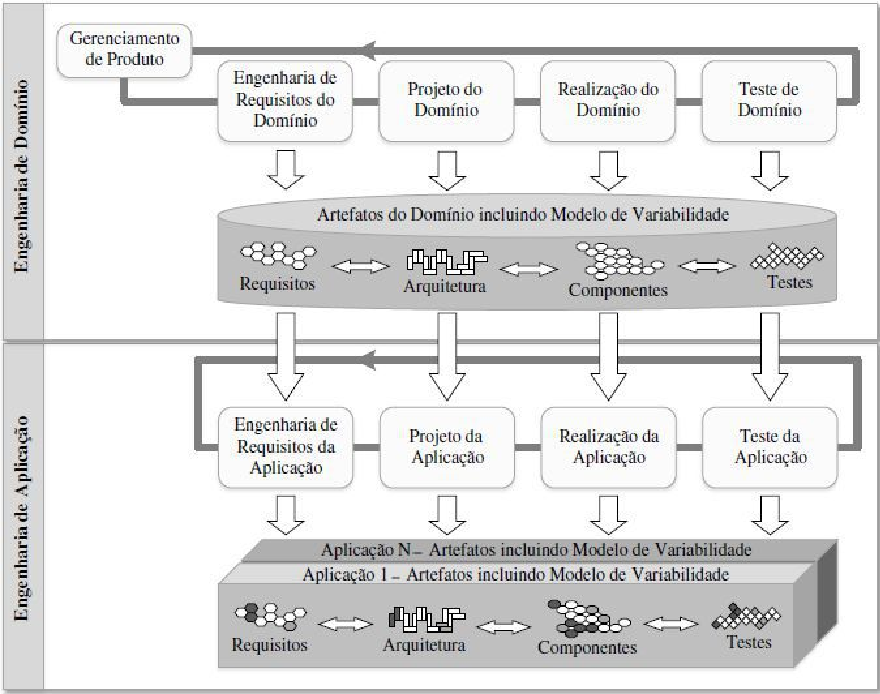
\includegraphics[scale=0.90]{lps.pdf}
	\caption{\textit{Framework} de Engenharia de LPS, traduzido de \citet{pohl2005software}}
	\label{fig:lps}
\end{figure}

Variabilidades são descritas por: Ponto de Variação, que permite a resolução de variabilidades em artefatos genéricos de uma LPS; Variante, que representa os possíveis elementos que podem ser escolhidos para resolver um ponto de variação e; Restrições entre variantes que estabelecem os relacionamentos entre uma ou mais variantes com o objetivo de resolver seus respectivos pontos de variação ou variabilidade em um dado tempo de resolução \cite{linden2007product, pohl2005software, apel2016feature}.

Existem abordagens voltadas para o gerenciamento de variabilidade, especialmente as baseadas em UML. Dentre as quais, pode-se citar a \textit{Product Line UML-based Software Engineering} (PLUS) \cite{gomaa2006designing} e a \textit{Stereotype-based Management of Variability} (\textit{SMarty}) \cite{junior2010systematic}.

Neste trabalho considera-se \textit{SMarty}, que realiza o gerenciamento de variabilidades de uma LPS fazendo uso de diagramas UML, e é composta de um perfil UML denominado \textit{SMartyProfile} e de um processo denominado \textit{SMartyProcess}. 

\textit{SMarty} guia o usuário por meio do \textit{SMartyProcess} na identificação e representação de variabilidades de uma LPS. O perfil \textit{SMartyProfile} é formado por um conjunto de estereótipos e meta-atributos para representar variabilidades em modelos UML de LPS.

O \textit{SMartyProfile} permite ao usuário a aplicação dos estereótipos de forma clara e objetiva \cite{junior2010systematic,junior2013systematic,fiori2012variability} e se baseia no inter-relacionamento dos principais conceitos de LPS no que tange ao gerenciamento de variabilidade. Tais conceitos são aplicados aos elementos de interesse do metamodelo da UML. Com base no relacionamento entre os conceitos de gerenciamento de variabilidade e os modelos UML, a \ref{fig:smartyprofile} apresenta o perfil UML \textit{SMartyProfile} 5.1.



O núcleo de artefatos forma a base da LPS e inclui a arquitetura de LPS, componentes reusáveis, modelos de domínios, requisitos da LPS, planos de testes e modelos de características (\textit{features}) e de variabilidades.


\begin{landscape}
	
	\begin{figure}[h!]
		\centering
		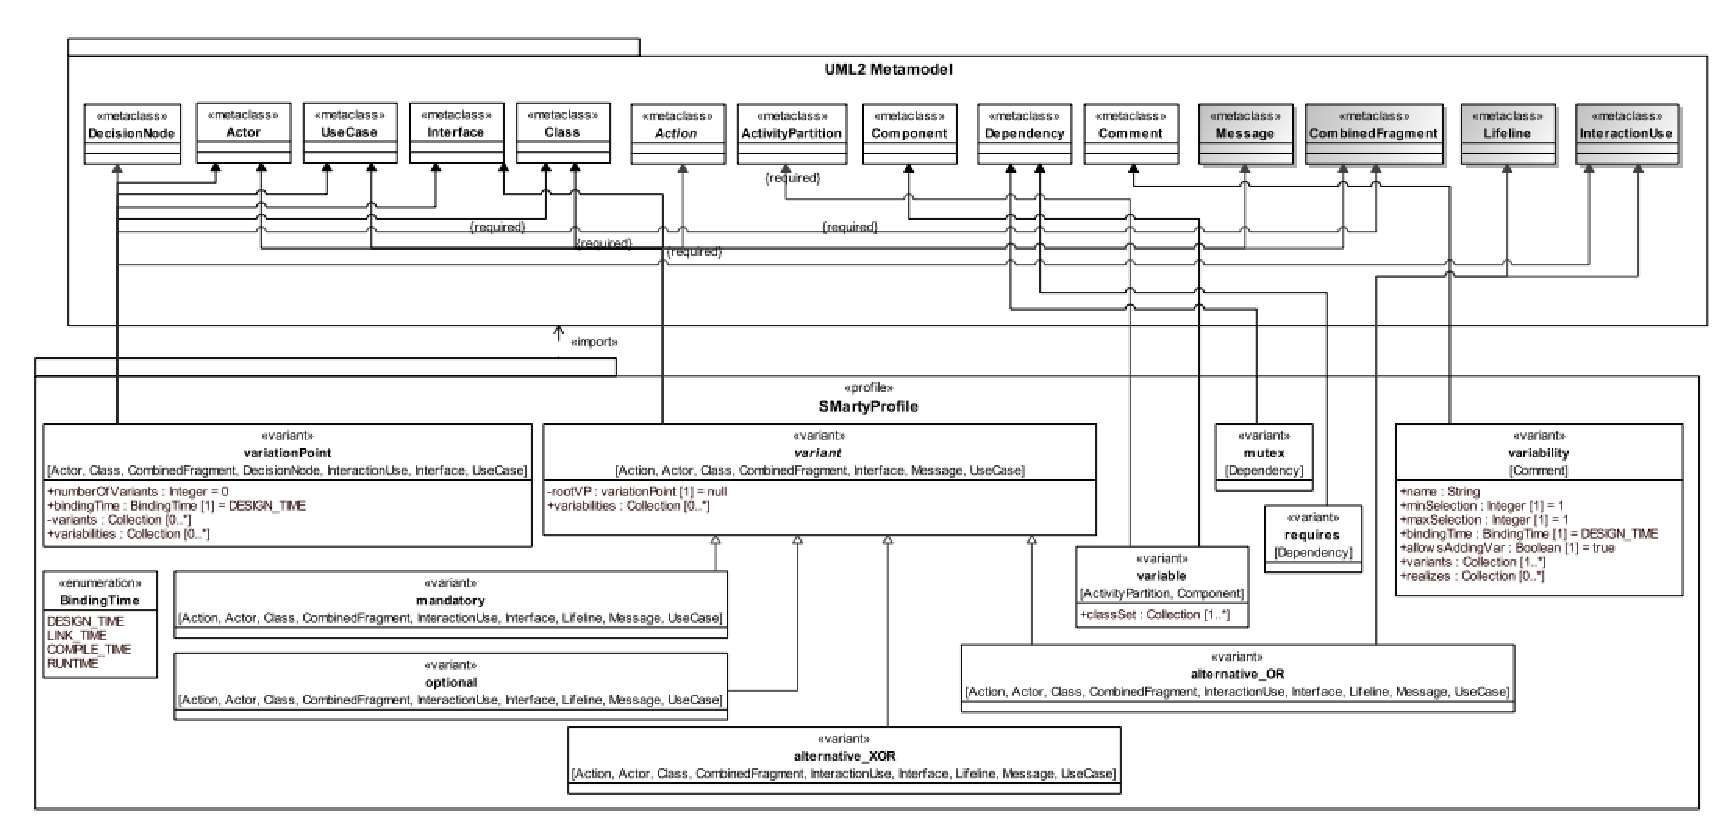
\includegraphics[scale=0.80]{smartyprofile.pdf}
		\caption{ Estereótipos e Meta-Atributos do Perfil \textit{SMartyProfile} 5.2 com Suporte a Diagramas de Casos de Uso, Classes, Componentes, Atividades e Sequência \cite{bera2015evidence}}
		\label{fig:smartyprofile}
	\end{figure}
	
	
\end{landscape}

O \textit{SMartyProcess} é um processo sistemático que guia o usuário na identificação, delimitação, representação, rastreamento de variabilidades e análise de configurações de produtos de uma LPS e segue as atividades gerais relacionadas às especificadas no processo de desenvolvimento de LPS \cite{pohl2005software}. Tal relacionamento pode ser observado por meio da \ref{fig:smartyprocess}, em um diagrama de atividades da UML. Nela é possível observar o processo genérico de Desenvolvimento de Linha de Produto, representado pelas atividades alinhadas no lado esquerdo e o \textit{SMartyProcess} representado pelas atividades do retângulo à direita \cite{de2005variability}. Mais informações relacionadas à \textit{SMarty} podem ser encontradas no Anexo \ref{sec:Abordagem_SMarty} - Abordagem \textit{SMarty}.


\begin{figure}[h!]
	\centering
	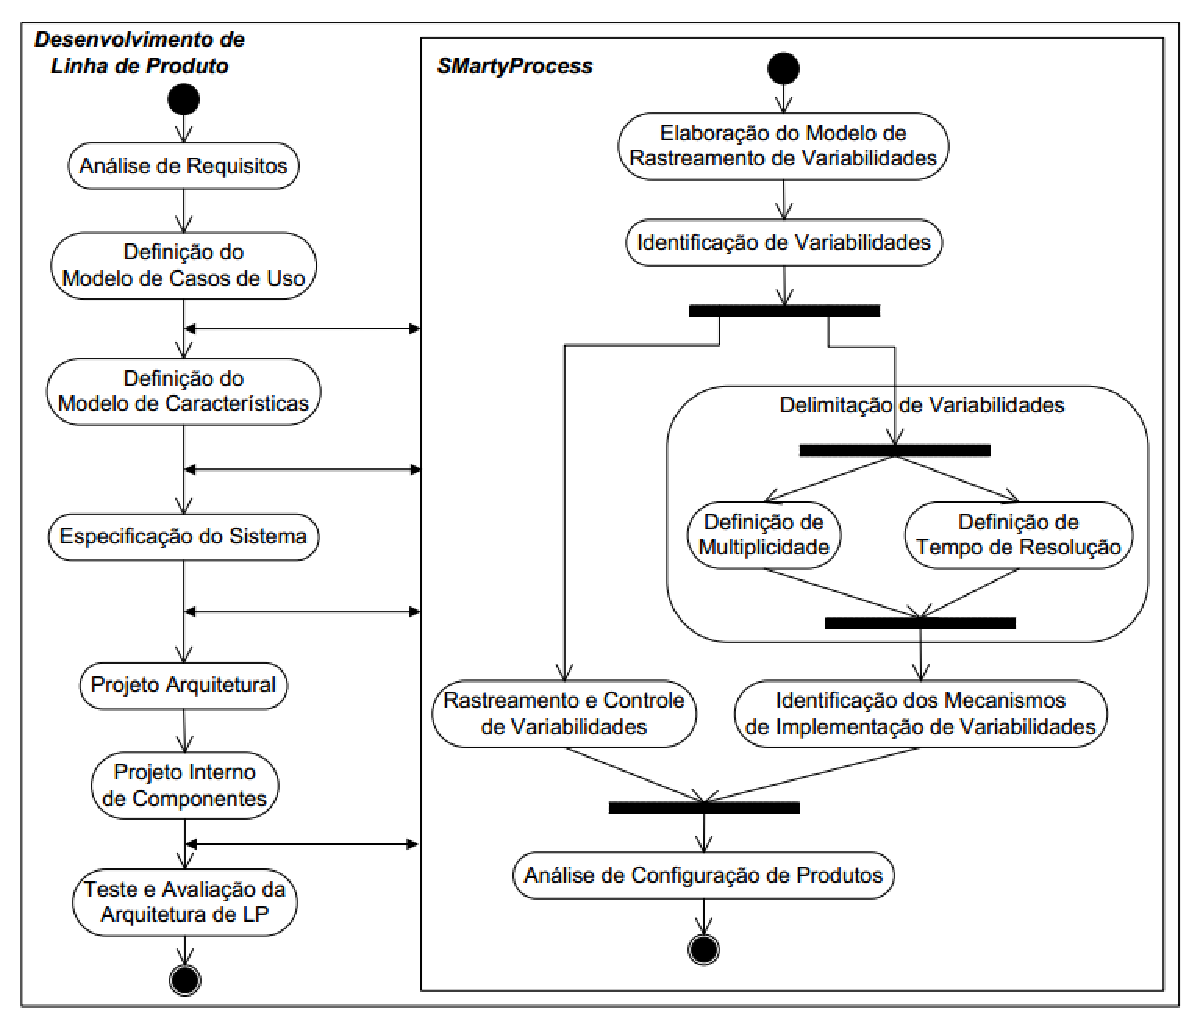
\includegraphics[scale=0.60]{smartyprocess.pdf}
	\caption{ O Processo de Gerenciamento de Variabilidades \textit{SMartyProcess} e sua Interação entre as Atividades com o Processo de Desenvolvimento de LPS, traduzido de \citet{de2005variability}}
	\label{fig:smartyprocess}
\end{figure}

Na \ref{fig:usecase} é apresentado um diagrama de casos de uso da LPS \textit{Arcade Game Maker} (AGM) \cite{seiagm} contendo notações de variabilidade modeladas de acordo com \textit{SMarty}.

\begin{figure}[h!]
	\centering
	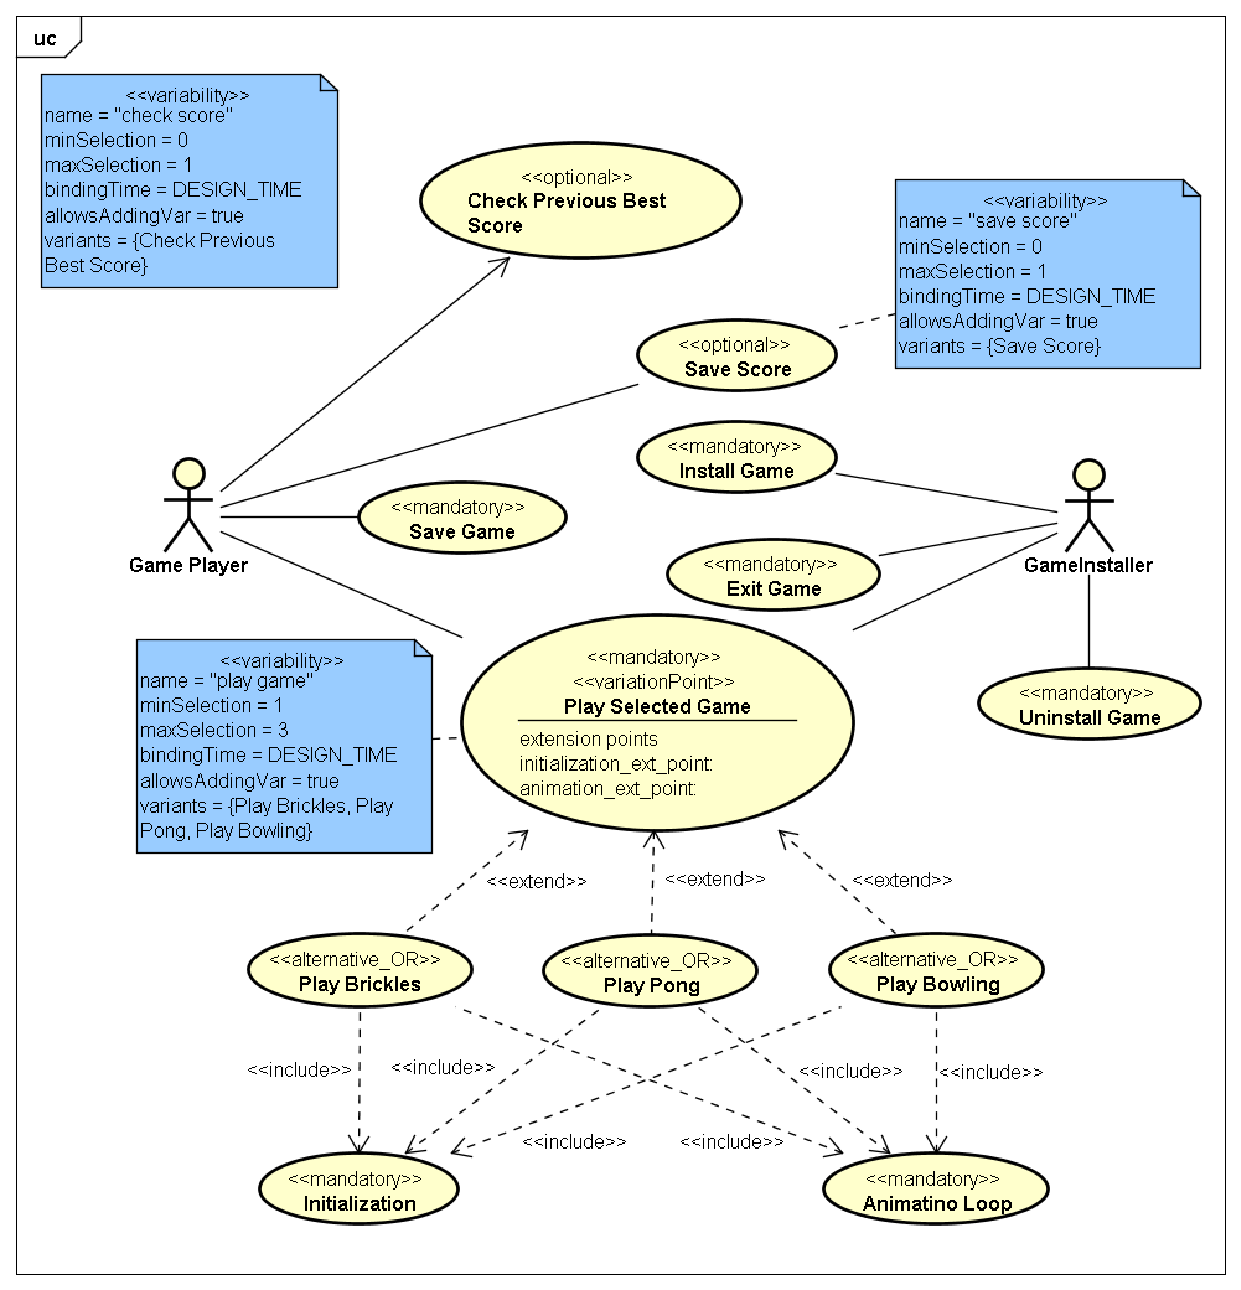
\includegraphics[scale=0.60]{UC_AGM.pdf}
	\caption{Diagrama de casos de uso da LPS AGM contendo as notações \textit{SMarty} \cite{MarcolinoSEKE2013}}
	\label{fig:usecase}
\end{figure}

Na \ref{fig:usecase} pode-se perceber que existem representações de esteriótipos com itens representando a variabilidade. Para a representação do ponto de variação tem-se \textit{variationPoint} ou ponto de variação e a \textit{variability} ou variabilidade, outros estereótipos são representados, contudo, para entendimento de variabilidade esses dois são essenciais.

O primeiro, ponto de variação, é a resolução de variabilidades em artefatos genéricos de uma LPS, a variabilidade representa os possíveis elementos pelos quais um ponto de variação pode ser resolvido e também pode representar uma maneira de resolver uma variabilidade diretamente.    



\section{Teste de Linha de Produto de Software}
\label{cap2sec:teste_lps}

O potencial de reuso de artefatos além de aumentar a produtividade torna a LPS atrativa ao mercado. Para alcançar as melhorias pretendidas, a qualidade dos artefatos reutilizáveis deve ser verificada. Teste de software ainda é a técnica de garantia de qualidade mais comum na indústria, no entanto, a evolução dos sistemas e o aumento da complexidade computacional vêm forçando a criação de processos e atividades mais complexas no que tange ao desenvolvimento de software em larga escala \cite{Apel:2013:FSP:2541773}. 

Teste de software é um processo que faz parte do desenvolvimento de software e tem como principal objetivo revelar defeitos para que sejam corrigidos até que o produto final atinja a qualidade desejada e satisfaça os seus requisitos. Isto porque o custo de reparo de falhas é maior ao final do desenvolvimento do que em estágios iniciais. Assim, antecipando-se os testes, o custo do produto se torna menor e se obtém um ganho em qualidade \cite{do2014strategies}.


As terminologias aplicadas ao contexto de teste de software que referem-se aos elementos de investigação podem ser definidas, segundo \citet{delamaro2017introduccao} da seguinte forma:


\begin{itemize}
	\item \textbf{Falha:} É um comportamento inesperado do software. Uma falha pode ter sido causada por diversos erros, mas alguns erros podem nunca causar uma falha.
	\item \textbf{Defeito:} É uma inconsistência no software, algo que foi implementado de maneira incorreta. Ocorre em uma linha de código, como uma instrução errada ou um comando incorreto. O defeito é a causa de um erro, porém, se uma linha de código que contém o defeito nunca for executada, o defeito não irá provocar erro.
	\item \textbf{Erro:} Erro humano produzindo resultado incorreto. O erro evidencia o defeito, ou seja, quando há diferença entre o valor obtido e o valor esperado constitui um erro.
\end{itemize}


Para que os objetivos da execução dos testes sejam alcançados, existe uma cadeia organizada de atividades, como na engenharia de software, em que um ciclo de vida perfaz todos os pontos necessários para se alcançar o objetivo final \cite{delamaro2017introduccao}. O ciclo de Vida dos Testes é composto de 5 fases segundo \citet{crespo2004metodologia}: Planejamento, Preparação, Especificação, Execução e Entrega (\ref{fig:testelps}).

\begin{figure}[h!]
	\centering
	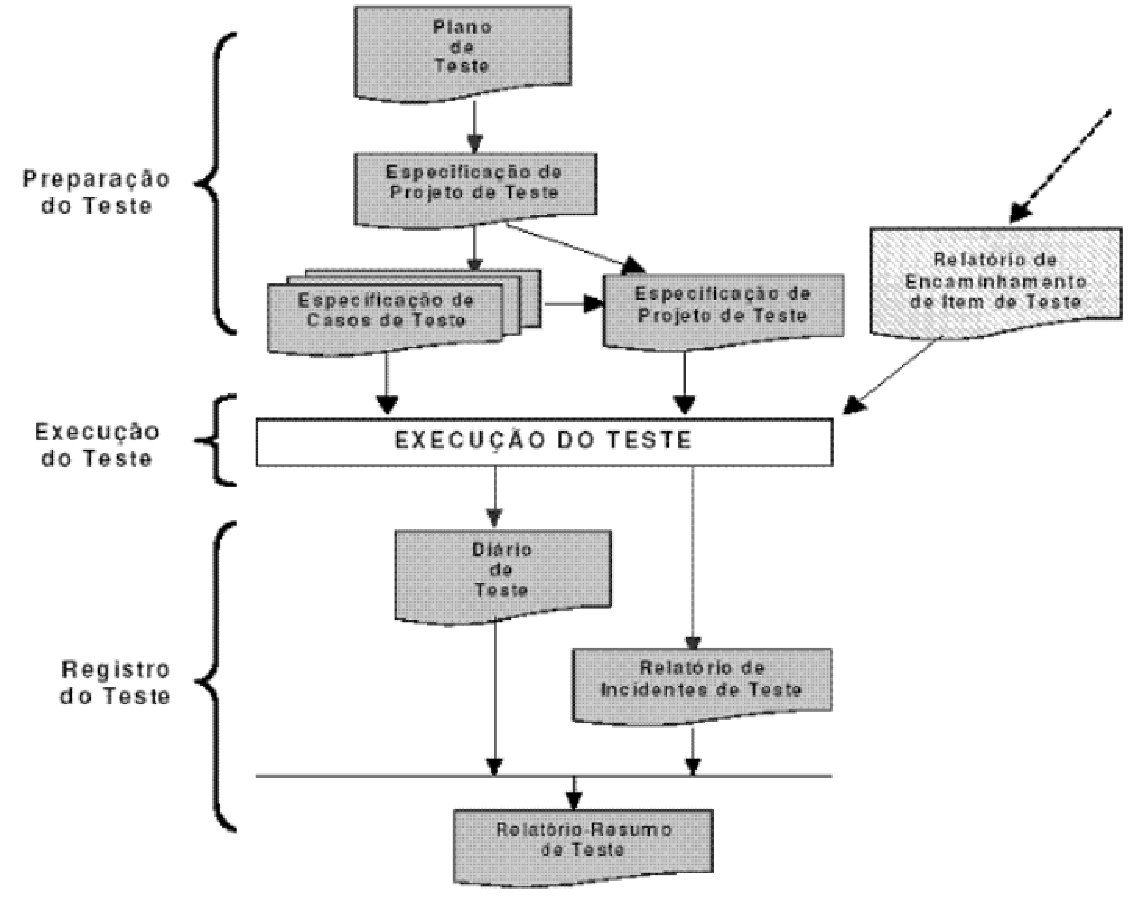
\includegraphics[scale=0.40]{testelps.pdf}
	\caption{Modelo de proposta de implantação do processo de teste de software segundo \citet{crespo2004metodologia}}
	\label{fig:testelps}
\end{figure}

Teste de LPS é um grande desafio por causa do amplo conjunto de produtos que podem ser derivados de um núcleo de artefatos comuns e suas variabilidades (\ref{fig:casotestelps}). Sendo assim, para uma pesquisa completa a respeito de teste em LPS, primeiro é necessário entender mais sobre o modelo de processo de teste. Um exemplo de ciclo de vida comumente utilizado no apoio ao teste é o modelo V (\ref{fig:testeV}).

\begin{figure}[h!]
	\centering
	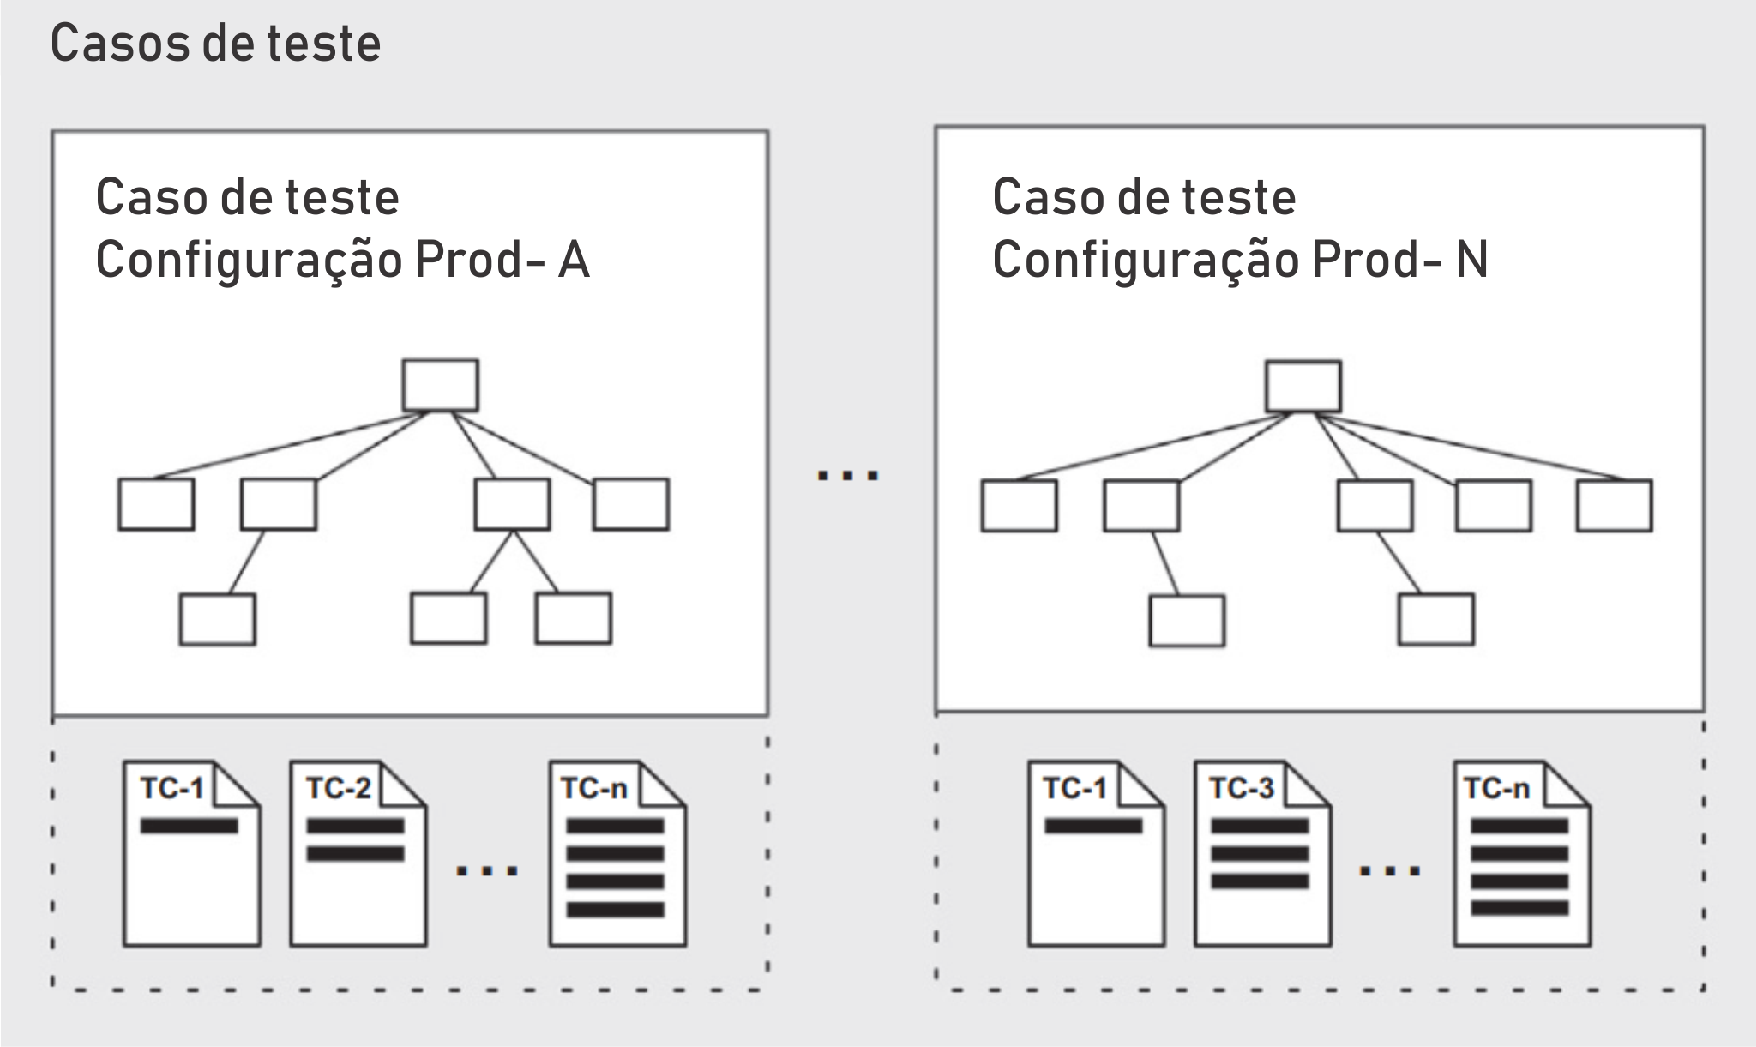
\includegraphics[scale=0.4]{casotestelps.pdf}
	\caption{ Representação de interesse em testes de SPL: seleção de instâncias do produto para testar. Traduzido de \citet{do2014strategies}}
	\label{fig:casotestelps}
\end{figure}

\begin{figure}[h!]
	\centering
	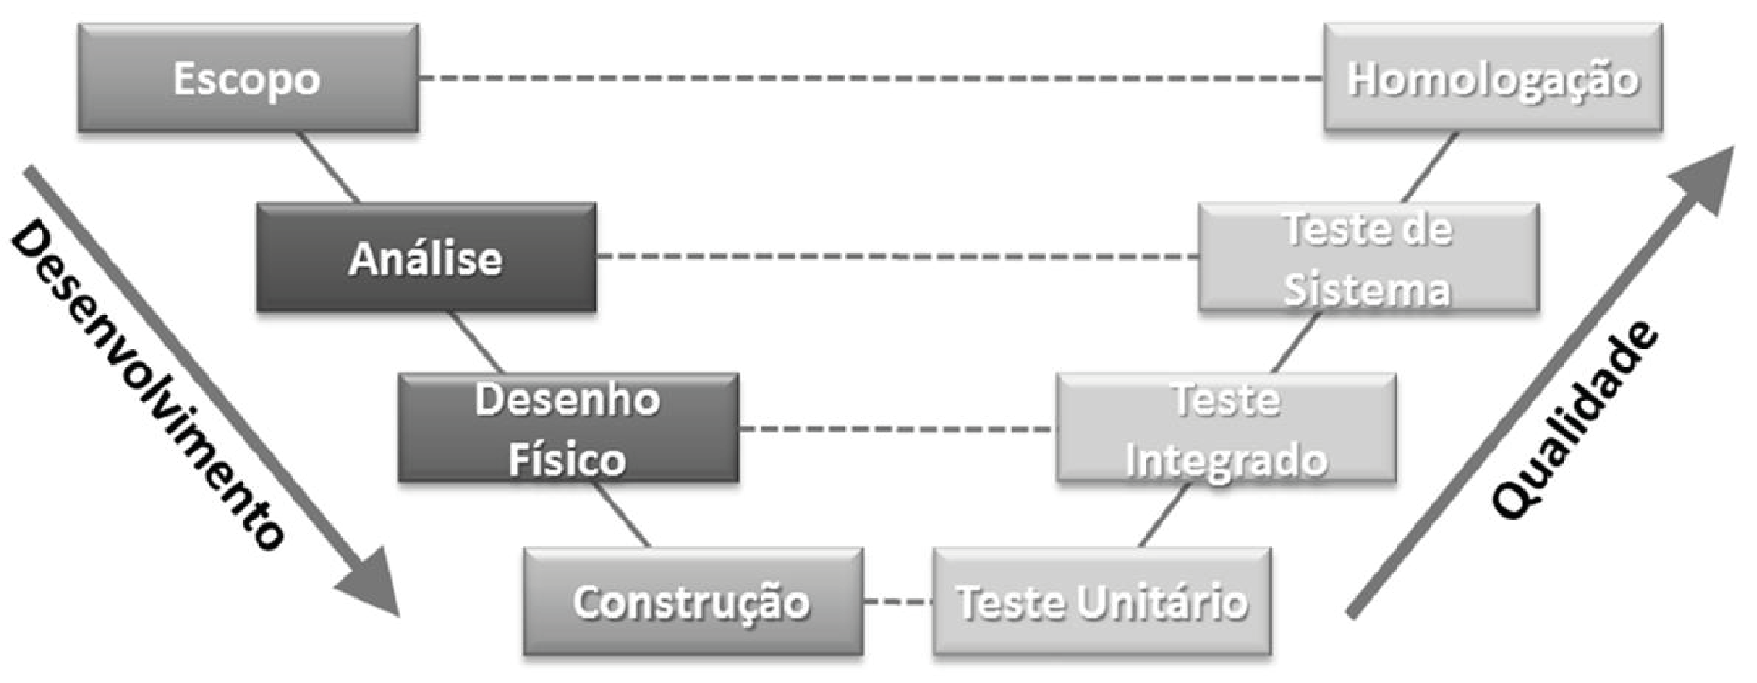
\includegraphics[scale=0.40]{teste.pdf}
	\caption{Esquema simplificado que representa o modelo V de gerenciamento de atividades de engenharia de sistemas. Traduzido de \citet{do2014strategies}}
	\label{fig:testeV}
\end{figure}

O modelo V de desenvolvimento é um modelo conceitual de Engenharia de sistemas/
desenvolvimento de produto, visto como melhoria ao problema de reatividade do modelo em cascata. E permite que, durante a integração de um sistema em seus diversos níveis, os testes sejam feitos contra os próprios requisitos do componente/interface que está sendo testado(a), em contraste com modelos anteriores em que o componente era testado contra a especificação do componente/interface.

Como mencionado anteriormente, o desafio na geração e execução de teste em LPS, se deve principalmente à geração de produtos derivados do núcleo de artefatos comuns e suas variabilidades (vide Seção \ref{cap2sec:lps}). Isso porque, para cada instanciação de produto na LPS, casos de teste já existentes podem não ser mais aplicados por causa da variação das funcionalidades (\ref{fig:casotestelps}). 

\citet{do2014strategies} apresentam algumas abordagens que visam à diminuição dessa lacuna na geração e execução de teste para produtos derivados de LPS. Demonstram também que TBM vem se apresentando como uma alternativa à geração antecipada de casos de teste considerando variações de produtos, isso porque a geração da sequência ou casos de teste se dá durante a criação dos modelos na engenharia de domínio de LPS. 


\section{Teste Baseado em Modelos para LPS}
\label{cap2sec:teste_tbm_lps}

Teste Baseado em Modelo (TBM) tem como característica principal o fato de ser uma abordagem de teste caixa preta, derivada de um modelo que descreve aspectos funcionais do produto testado. Também se refere a um processo de engenharia de software que estuda, constrói, analisa e aplica modelos bem definidos para dar suporte às atividades relacionadas com testes \cite{shafique2010systematic}.

TBM tem por objetivo verificar se a especificação de um software está de acordo com o seu modelo e foca na geração automática de sequências ou casos de testes. A ideia básica é identificar e construir um modelo abstrato que represente o comportamento do \textit{System Under Test} (SUT). Com esse modelo é possível gerar um grande número de casos de teste ainda na modelagem do produto \cite{devroey2014behavioural}. 

Tais casos de testes, derivados dos modelos, são conhecidos como a suíte abstrata de testes, e seu nível de abstração está intimamente relacionado ao nível de abstração do modelo, segundo \citet{do2014strategies}. As vantagens da abordagem é que a geração de testes começa mais cedo no ciclo do desenvolvimento e podem ser criados casos de teste automaticamente a partir de um modelo. 

Os casos de teste podem ser representados por meio de árvores de decisão, \textit{statecharts}, ontologias de domínio ou diagramas de casos de uso e/ou estados da \textit{Unified Modeling Language} (UML) \cite{isa2017model}.

O processo de TBM (\ref{fig:tbm}) pode ser dividido em cinco passos:

\begin{enumerate}
	\item Modelar o SUT;
	\item Gerar os testes abstratos a partir do modelo;
	\item Transformar os testes abstratos em testes executáveis;
	\item Executar os testes no SUT;
	\item Analisar os resultados.
\end{enumerate}
 
 \begin{figure}[h!]
 	\centering
 	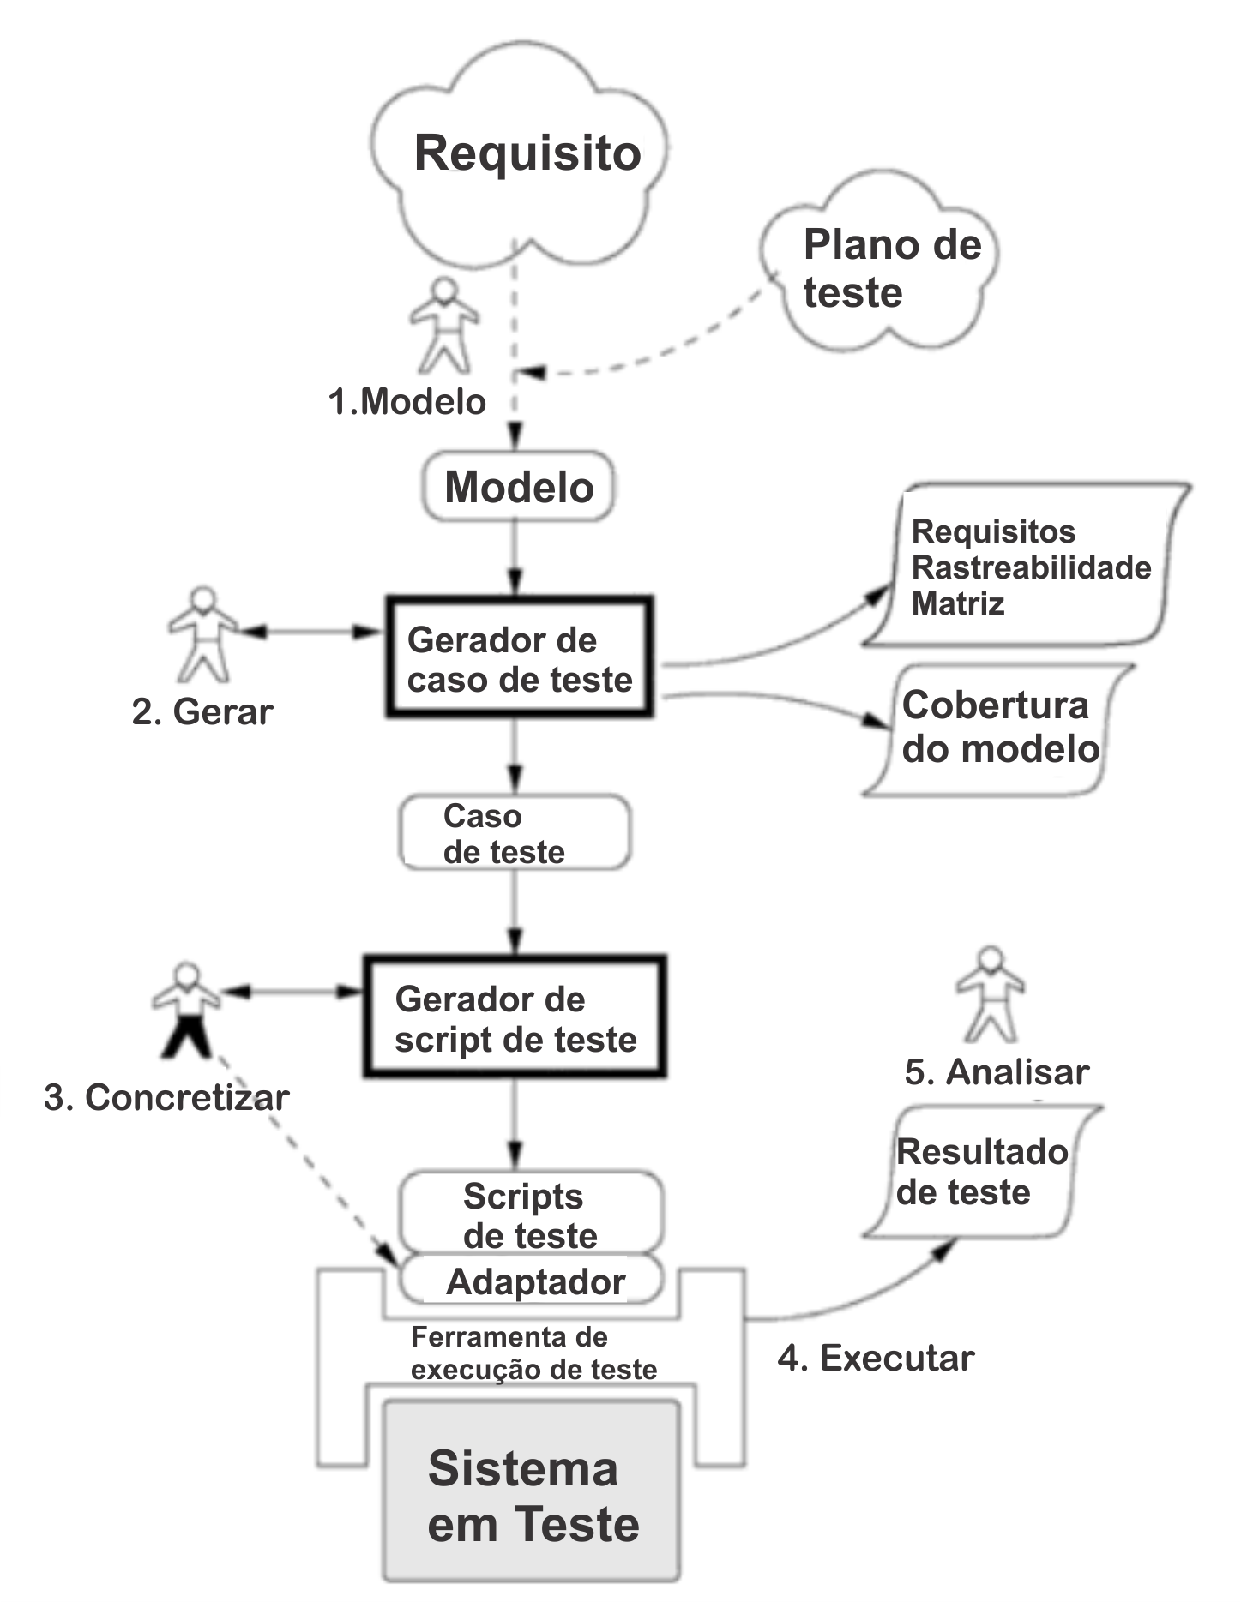
\includegraphics[scale=0.40]{tbm.pdf}
 	\caption{ Ciclo de Processo de TBM, Traduzido de \citet{utting2010practical}}
 	\label{fig:tbm}
 \end{figure}

\citet{do2014strategies} apontam que testes devem ser considerados na engenharia de domínio e na de aplicação. Dentro do interesse de teste, dois itens devem ser levados em consideração: o conjunto de requisitos do produto e a qualidade do modelo de variabilidade em teste. Esses autores apresentam também uma grande quantidade de trabalhos que apontam técnicas para lidar com o aspecto de seleção de produto para teste e o teste real dos produtos, utilizando TBM para LPS. No entanto, consideram a falta de relatos reais de experiências industriais que podem limitar algumas conclusões. O estudo ainda apresenta uma série de estratégias que podem apoiar a seleção e a execução dos testes reais em produtos.

Baseado nesse cenário, um dos maiores desafios em teste de LPS se dá em relação às particularidades de cada modelo. Para isso, TBM busca, na criação de modelos da engenharia de domínio, realizar a geração de casos de teste que possam ser reutilizados na engenharia de aplicação. Alguns trabalhos apresentados por \citet{do2014strategies} focam na construção da geração antecipada dos testes na modelagem de domínio de uma LPS.

Uma particularidade de TBM é que normalmente faz de uso de Máquinas de Estados Finitos (MEF) (\ref{fig:tbmmef}), um modelo formal que representa as possíveis configurações de um sistema.

\begin{figure}[h!]
	\centering
	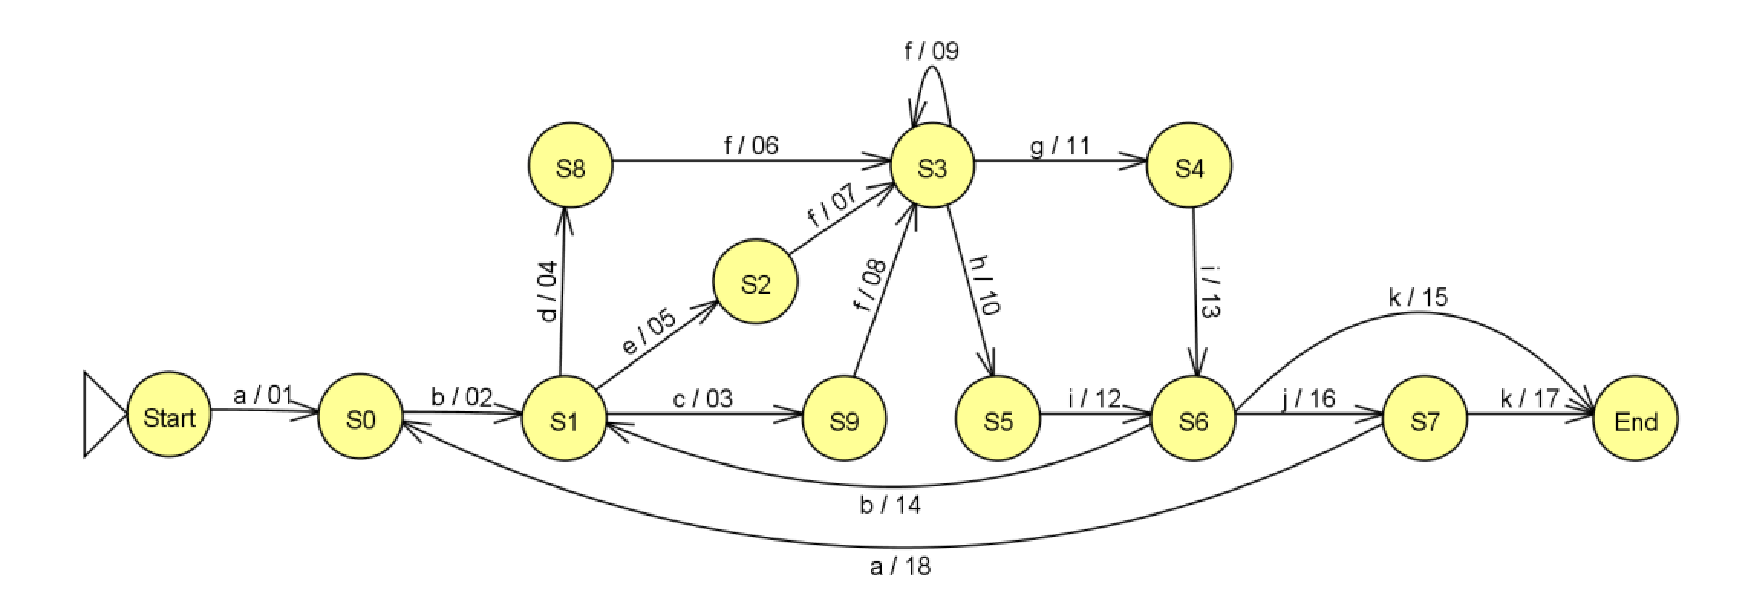
\includegraphics[scale=0.50]{fsm.pdf}
	\caption{ Exemplo de grafo de uma MEF \cite{costa2016split}}
	\label{fig:tbmmef}
\end{figure}

A \ref{fig:tbmmef} apresenta um exemplo MEF. Nela observam-se os estados (nós) e as suas transições (arestas). Esse modelo finito e formal permite melhor observação do comportamento das atividades do sistema modelado.

Sabendo que TBM possui particularidades em sua utilização em LPS e que proporciona, de certa forma, suporte à variabilidade, foi realizado um Mapeamento Sistemático da Literatura (MSL) (Apêncie \ref{sec:secmsl_MSL}), com a finalidade de evidenciar como TBM tem sido utilizado em LPS. 

Na \ref{tab:listaextraquali} são relacionados os 44 trabalhos analisados no MSL, por meio dos quais pode-se tirar conclusões e suposições para nortear este trabalho com relação:

\begin{itemize}
	\item aos principais diagramas utilizados;
	\item à utilização de ferramentas de apoio;
	\item às abordagens de teste utilizadas; e
	\item ao gerenciamento de variabilidade.
\end{itemize}

 Em seguida um mapa (\ref{fig:roadmap}) foi criado a partir da análise dos trabalhos do MSL. Tal mapa serve como um guia para direcionamento de estudos por temas de interesse. Esse direcionamento pode ser feito por assunto específico ou pelo caminho que um determinado estudo percorreu até o objetivo final, que é a geração de casos de teste.



\begin{landscape}
	\scalefont{0.6}
	\begin{longtable}[c]{c|l|l|c|c|c}
		\caption{Trabalhos selecionados para leitura e extração de dados do MSL}
		\label{tab:listaextraquali}\\
		\hline
		\textbf{ID} & \multicolumn{1}{c|}{\textbf{Título}} & \multicolumn{1}{c|}{\textbf{Autor(res)}} & \textbf{\begin{tabular}[c]{@{}c@{}}Ano de \\ Publicação\end{tabular}} & \textbf{Fonte} & \textbf{Tipo} \\ \hline
		\endfirsthead
		
		\hline
		\textbf{ID} & \multicolumn{1}{c|}{\textbf{Título}} & \multicolumn{1}{c|}{\textbf{Autor(res)}} & \textbf{\begin{tabular}[c]{@{}c@{}}Ano de \\ Publicação\end{tabular}} & \textbf{Fonte} & \textbf{Tipo} \\ \hline
		
		\endhead
		
		T1 & \begin{tabular}[c]{@{}l@{}}Delta-Oriented Model-Based \\ SPL Regression Testing\end{tabular} & \begin{tabular}[c]{@{}l@{}}Sascha Lity, Malte Lochau, \\ Ina Schaefer, Ursula Goltz\end{tabular} & 2012 & ACM & Evento \\ \hline
		T2 & \begin{tabular}[c]{@{}l@{}}Industrial Evaluation of Pairwise \\ SPL Testing with MoSo-PoLiTe\end{tabular} & \begin{tabular}[c]{@{}l@{}}Michaela Steffens, Sebastian Oster, \\ Malte Lochau, Thomas Fogdal\end{tabular} & 2012 & ACM & Evento \\ \hline
		T3 & \begin{tabular}[c]{@{}l@{}}Model-Based Coverage-Driven Test Suíte \\ Generation for Software Product Lines\end{tabular} & \begin{tabular}[c]{@{}l@{}}Harald Cichos, Sebastian Oster, \\ Malte Lochau, Andy Schurr\end{tabular} & 2011 & ACM & Periódico \\ \hline
		T4 & \begin{tabular}[c]{@{}l@{}}MoSo-PoLiTe - Tool Support for \\ Pairwise and Model-Based Software \\ Product Line Testing\end{tabular} & \begin{tabular}[c]{@{}l@{}}Sebastian Oster, Ivan Zorcic, \\ Florian Markert, Malte Lochau\end{tabular} & 2011 & ACM & Evento \\ \hline
		T5 & MPLM - MaTeLo Product Line Manager & Hamza Samih, Ralf Bogusch & 2014 & ACM & Evento \\ \hline
		T6 & \begin{tabular}[c]{@{}l@{}}On the use of test cases in model-based \\ software product line development\end{tabular} & \begin{tabular}[c]{@{}l@{}}Alexander Knapp, Markus Roggenbach, \\ Bernd-Holger Schlingloff\end{tabular} & 2014 & ACM & Evento \\ \hline
		T7 & \begin{tabular}[c]{@{}l@{}}Pairwise Feature-Interaction Testing \\ for SPLs: Potentials and Limitations\end{tabular} & \begin{tabular}[c]{@{}l@{}}Sebastian Oster, Malte Lochau, \\ Marius Zink, Mark Grechanik\end{tabular} & 2011 & ACM & Evento \\ \hline
		T8 & \begin{tabular}[c]{@{}l@{}}Deriving Usage Model Variants for \\ Model- based Testing: An Industrial Case Study\end{tabular} & \begin{tabular}[c]{@{}l@{}}Hamza Samih,  Hélène Le Guen, \\ Ralf Bogusch, Mathieu Acher, Benoit Baudry\end{tabular} & 2014 & IEEE & Evento \\ \hline
		T9 & \begin{tabular}[c]{@{}l@{}}Model-based Software Product Line \\ Testing by Coupling Feature Models \\ with Hierarchical Markov Chain Usage Models\end{tabular} & Ceren Sahin Gebizli, Hasan Sozer & 2016 & IEEE & Evento \\ \hline
		T10 & \begin{tabular}[c]{@{}l@{}}Model-Based Test Design of Product Lines: \\ Raising Test Design to the Product Line Level\end{tabular} & \begin{tabular}[c]{@{}l@{}}Hartmut Lackner, Martin Thomas, \\ Florian Wartenberg, Stephan Weißleder\end{tabular} & 2014 & IEEE & Periódico \\ \hline
		T11 & Requirements-Based Delta-Oriented SPL Testing & \begin{tabular}[c]{@{}l@{}}Michael Dukaczewski, Ina Schaefer, \\ Remo Lachmann, Malte Lochau\end{tabular} & 2013 & IEEE & Evento \\ \hline
		T12 & \begin{tabular}[c]{@{}l@{}}Using Feature Model to Support Model- Based \\ Testing of Product Lines: An Industrial Case Study\end{tabular} & \begin{tabular}[c]{@{}l@{}}Shuai Wang,  Shaukat Ali,\\  Tao Yue, Marius Liaaen\end{tabular} & 2013 & IEEE & Periódico \\ \hline
		T13 & \begin{tabular}[c]{@{}l@{}}An automated Model-based Testing \\ Approach in Software Product Lines \\ Using a Variability Language\end{tabular} & \begin{tabular}[c]{@{}l@{}}Boni García,  Rodrigo García-Carmona, \\ Álvaro Navas, Hugo A. Parada-Gélvez,\\  Félix Cuadrado, Juan C. Dueñas\end{tabular} & 2010 & \begin{tabular}[c]{@{}c@{}}Politécnica \\ Arquivo \\ digital UPM\end{tabular} & Evento \\ \hline
		T14 & \begin{tabular}[c]{@{}l@{}}Automated Product Line Methodologies \\ to Support Model-Based Testing\end{tabular} & Shuai Wang,  Shaukat Ali, Arnaud Gotlieb & 2013 & \begin{tabular}[c]{@{}c@{}}CEUR \\ Event Proceedings\end{tabular} & Evento \\ \hline
		T15 & \begin{tabular}[c]{@{}l@{}}Behavioural Model Based \\ Testing of Software Product Lines\end{tabular} & Xavier Devroey & 2014 & ACM & Evento \\ \hline
		T16 & \begin{tabular}[c]{@{}l@{}}Feature Model-based \\ Software Product Line Testing\end{tabular} & Sebastian Oster & 2012 & TUprints & Periódico \\ \hline
		T17 & \begin{tabular}[c]{@{}l@{}}Model-based pairwise testing for feature interaction \\ coverage in software product line engineering\end{tabular} & \begin{tabular}[c]{@{}l@{}}Malte Lochau, Sebastian Oster, \\ Ursula Goltz, Andy Schurr\end{tabular} & 2011 & Springer & Periódico \\ \hline
		T18 & Model-based Test Generation for Software Product Line & Xinying Cai, Hongwei Zeng & 2013 & IEEE & Evento \\ \hline
		T19 & Model-Based Testing for Software Product Lines & Erika Mir Olimpiew & 2008 & Springer & Evento \\ \hline
		T20 & PLETS - A Product line of model-based testing tools & Elder de Macedo Rodrigues & 2013 & PUC-RS & Evento \\ \hline
		T21 & \begin{tabular}[c]{@{}l@{}}Top-Down and Bottom-Up Approach for \\ Model-Based Testing of Product Lines\end{tabular} & Stephan Weißleder, Hartmut Lackner & 2013 & EPTCS & Evento \\ \hline
		T22 & \begin{tabular}[c]{@{}l@{}}A Product Line Modeling and Configuration  Methodology \\ to Support Model-Based  Testing: An Industrial Case Study\end{tabular} & \begin{tabular}[c]{@{}l@{}}Shaukat Ali, Tao Yue, Lionel Briand, \\ Suneth Walawege\end{tabular} & 2012 & Springer & Periódico \\ \hline
		T23 & \begin{tabular}[c]{@{}l@{}}Coverage Criteria for Behavioural \\ Testing of Software Product Lines\end{tabular} & \begin{tabular}[c]{@{}l@{}}Xavier Devroey, Gilles Perrouin, \\ Axel Legay, Maxime Cordy, \\ Pierre-Yves Schobbens, Patrick Heymans\end{tabular} & 2014 & Springer & Evento \\ \hline
		T24 & \begin{tabular}[c]{@{}l@{}}A Model Based Testing Approach for Model-Driven \\ Development and Software Product Lines\end{tabular} & \begin{tabular}[c]{@{}l@{}}Beatriz Pérez Lamancha,  Macario Polo Usaola, \\ Mario Piattini Velthius\end{tabular} & 2010 & Springer & Evento \\ \hline
		T25 & \begin{tabular}[c]{@{}l@{}}A Vision for Behavioural Model-Driven \\ Validation of Software Product Lines\end{tabular} & \begin{tabular}[c]{@{}l@{}}Xavier Devroey, Maxime Cordy,  \\ Gilles Perrouin, Eun-Young Kang, \\ Pierre-Yves Schobbens, Patrick Heymans, \\ Axel Legay,  Benoit Baudry\end{tabular} & 2012 & Springer & Evento \\ \hline
		T26 & \begin{tabular}[c]{@{}l@{}}Abstract Test Case Generation for Behavioural \\ Testing of Software Product Lines\end{tabular} & \begin{tabular}[c]{@{}l@{}}Xavier Devroey, Gilles Perrouin, \\ Pierre-Yves Schobbens\end{tabular} & 2014 & ACM & Evento \\ \hline
		T27 & \begin{tabular}[c]{@{}l@{}}Applying Incremental Model Slicing to \\ Product-Line Regression Testing\end{tabular} & \begin{tabular}[c]{@{}l@{}}Sascha Lity, Thomas Morbach,  \\ Thomas Th¨ um, Ina Schaefer\end{tabular} & 2016 & Springer & Periódico \\ \hline
		T28 & \begin{tabular}[c]{@{}l@{}}Automated Testing of Software-as- a-Service \\ Configurations using a Variability Language\end{tabular} & Sachin Patel, Vipul Shah & 2015 & ACM & Evento \\ \hline
		T29 & Delta-Oriented FSM-Based Testing & \begin{tabular}[c]{@{}l@{}}Mahsa Varshosaz,  Harsh Beohar, \\ Mohammad Reza Mousavi\end{tabular} & 2015 & Springer & Evento \\ \hline
		T30 & \begin{tabular}[c]{@{}l@{}}Incremental Model-Based Testing of \\ Delta-oriented Software Product Lines\end{tabular} & \begin{tabular}[c]{@{}l@{}}Malte Lochau, Ina Schaefer, \\ Jochen Kamischke, Sascha Lity\end{tabular} & 2012 & Springer & Periódico \\ \hline
		T31 & Model Based Testing in Software Product Lines & \begin{tabular}[c]{@{}l@{}}Pedro Reales, Macario Polo, \\ Danilo Caivano\end{tabular} & 2011 & Springer & Evento \\ \hline
		T32 & Model-Based Testing & \begin{tabular}[c]{@{}l@{}}Malte Lochau, Sven Peldszus, \\ Matthias Kowal,  Ina Schaefer\end{tabular} & 2014 & Springer & Evento \\ \hline
		T33 & \begin{tabular}[c]{@{}l@{}}Parameterized Preorder Relations for \\ Model-Based Testing of Software Product Lines\end{tabular} & Malte Lochau, Jochen Kamischke & 2012 & Springer & Evento \\ \hline
		T34 & Poster: VIBeS, Transition System Mutation Made Easy & \begin{tabular}[c]{@{}l@{}}Xavier Devroey, Gilles Perrouin, \\ Pierre-Yves Schobbens, Patrick Heymans\end{tabular} & 2015 & IEEE & Evento \\ \hline
		T35 & Spinal Test Suites for Software Product Lines & Harsh Beohar, Mohammad Reza Mousavi & 2014 & EPTCS & Evento \\ \hline
		T36 & \begin{tabular}[c]{@{}l@{}}Automated model-based testing\\ using the  UML testing profile and QVT\end{tabular} & \begin{tabular}[c]{@{}l@{}}Beatriz Pérez Lamancha, Pedro Reales Mateo, \\ IgnacioRodríguez de Guzmán, Macario Polo Usaola, \\ Mario Piattini Velthius\end{tabular} & 2009 & ACM & Evento \\ \hline
		T37 & \begin{tabular}[c]{@{}l@{}}Relating Variability Modeling and \\ Model- Based Testing for Software Product Lines Testing\end{tabular} & Hamza Samih & 2012 & ICTSS & Evento \\ \hline
		T38 & \begin{tabular}[c]{@{}l@{}}An Evaluation of Model-Based \\ Testing in Embedded Applications\end{tabular} & Stephan Weißleder, Holger Schlingloff & 2014 & IEEE & Evento \\ \hline
		T39 & \begin{tabular}[c]{@{}l@{}}Assessing Software Product Line Testing Via Model-Based \\ Mutation An Application to Similarity Testing\end{tabular} & \begin{tabular}[c]{@{}l@{}}Christopher Henard, Mike Papadakis, \\ Gilles Perrouin, Jacques Klein, Yves Le Traon\end{tabular} & 2013 & IEEE & Evento \\ \hline
		T40 & \begin{tabular}[c]{@{}l@{}}Automated and Scalable T-wise Test Case Generation \\ Strategies for Software Product Lines\end{tabular} & \begin{tabular}[c]{@{}l@{}}Gilles Perrouin, Sagar Sen, Jacques Klein, \\ Benoit Baudry, Yves le Traon Lassy\end{tabular} & 2010 & IEEE & Evento \\ \hline
		T41 & \begin{tabular}[c]{@{}l@{}}Model-based Testing of System Requirements \\ using UML Use Case Models\end{tabular} & Bill Hasling, Helmut Goetz, Klaus Beetz & 2008 & IEEE & Evento \\ \hline
		T42 & \begin{tabular}[c]{@{}l@{}}Successive refinement of models for model-based \\ testing to increase system test effectiveness\end{tabular} & \begin{tabular}[c]{@{}l@{}}Ceren Sahin Gebizli, Hasan Sozer, \\ Ali Ozer Ercan\end{tabular} & 2016 & IEEE & Evento \\ \hline
		T43 & A Software Product Line for Model-Based Testing Tools & \begin{tabular}[c]{@{}l@{}}Elder M. Rodrigues, Avelino F. Zorzo, \\ Itana M. Gimenez, Elisa Y. Nakagawa, \\ Flavio M. Oliveira, José C. Maldonado\end{tabular} & 2012 & PUC-RS & Outro \\ \hline
		T44 & \begin{tabular}[c]{@{}l@{}}Reusing State Machines for Automatic \\ Test Generation in Product Lines\end{tabular} & \begin{tabular}[c]{@{}l@{}}Stephan Weißleder, Dehla Sokenou, \\ Bernd-Holger Schlingloff\end{tabular} & 2008 & MoTip & Evento \\ \hline
	\end{longtable}
\end{landscape}



\begin{landscape}
	\begin{figure}[h!]
		\centering
		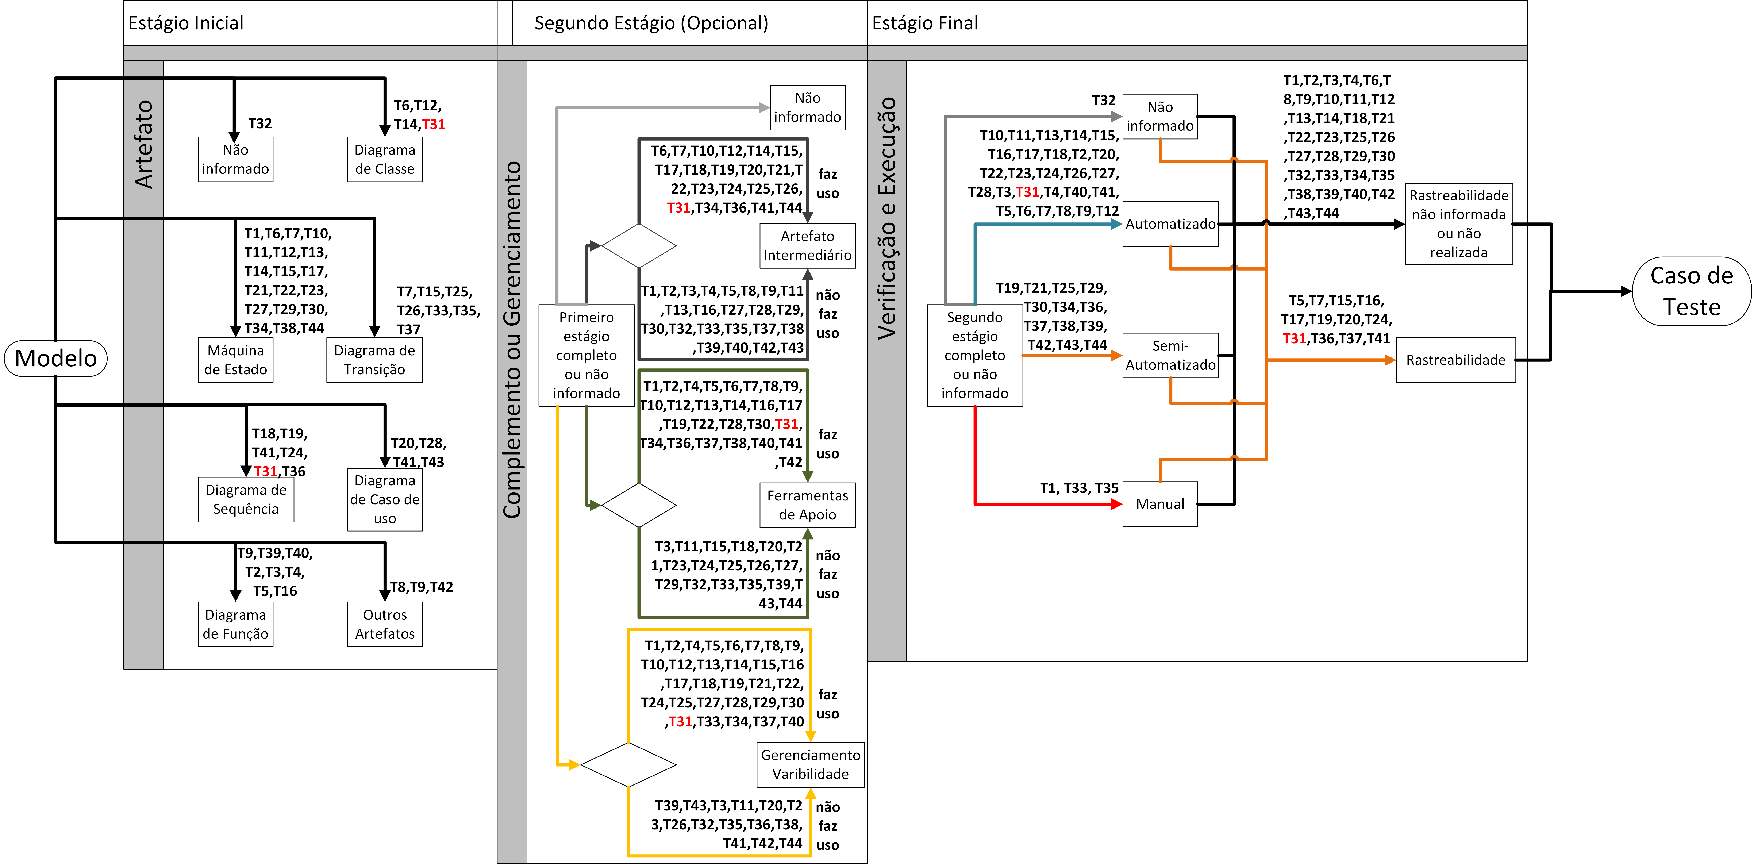
\includegraphics[scale=0.80]{roadmap.pdf}
		\caption{Mapeamento dos trabalhos relacionados ao TBM em LPS}
		\label{fig:roadmap}
	\end{figure}
\end{landscape}


\section{A Abordagem SPLiT-MBt}
\label{cap2sec:split_abordagem}

\citet{costa2016split} desenvolveu uma abordagem denominada \textit{Software Product Line Testing Method Based on System Models} (SPLiT-MBt) em que é possível gerar casos de teste e \textit{scripts} para testar os produtos derivados de uma LPS, com base no reuso inerente à LPS.

O método SPLiT-MBt suporta a geração automática de casos de teste funcionais a partir de diagramas de atividades da UML, mas pode ser expandido para outros modelos. A ideia é gerar artefatos de teste durante a engenharia de domínio e reutilizá-los durante a engenharia de aplicação. A \ref{fig:splitmbt} apresenta as etapas da abordagem SPLiT-MBt. 

\begin{figure}[h!]
	\centering
	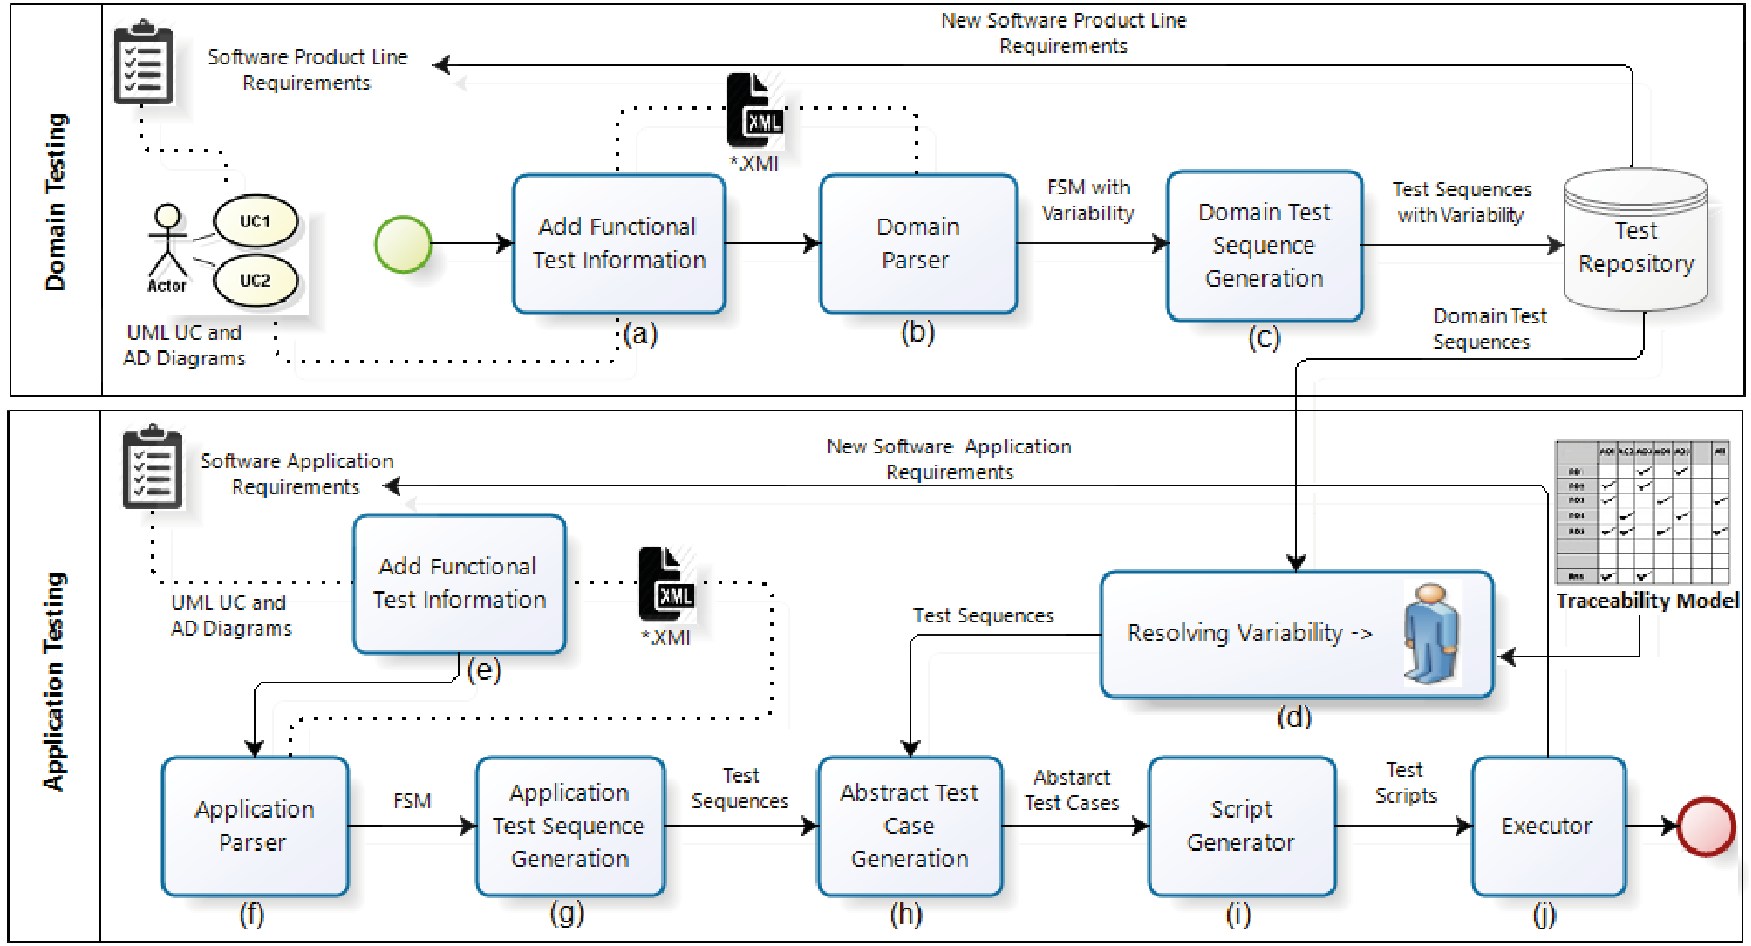
\includegraphics[width=\textwidth]{splitmbt.pdf}
	\caption{A abordagem SPLiT-MBt por \citet{costa2016split}}
	\label{fig:splitmbt}
\end{figure}

A abordagem é aplicada em duas etapas: primeiro, adicionam-se informações de teste nos modelos UML que foram projetados anteriormente, usando uma abordagem de gerenciamento de variabilidade para gerar sequências de teste durante a engenharia de domínio, no caso SPLiT-MBt faz uso da abordagem \textit{SMarty}. Segundo, adicionam-se informações de teste em modelos UML (durante a Engenharia de Aplicação) e resolve-se a variabilidade presente nas sequências de teste. 

O principal objetivo da abordagem é prover o reuso de artefatos de teste, baseado na adaptação do uso de TBM para se obter a geração automática de casos de teste funcional e \textit{scripts} para modelos, considerando a variabilidade das instâncias da LPS.

Na primeira etapa é realizada a anotação das informações de variabilidade e teste em modelos de sistema, aqui exemplificado por um diagrama de atividades na \ref{fig:costa1}. Em seguida, tais anotações são utilizadas para gerar sequências de teste fazendo uso de métodos de geração, no caso o \textit{Harmonized State Identifiers} (HSI) (Seção \ref{cap2subsubsec:hsi}). O modelo formal utilizado é a Máquina de Estados Finitos estendida para lidar com as informações sobre variabilidade, pontos de variação e variante.

\begin{figure}[h!]
	\centering
	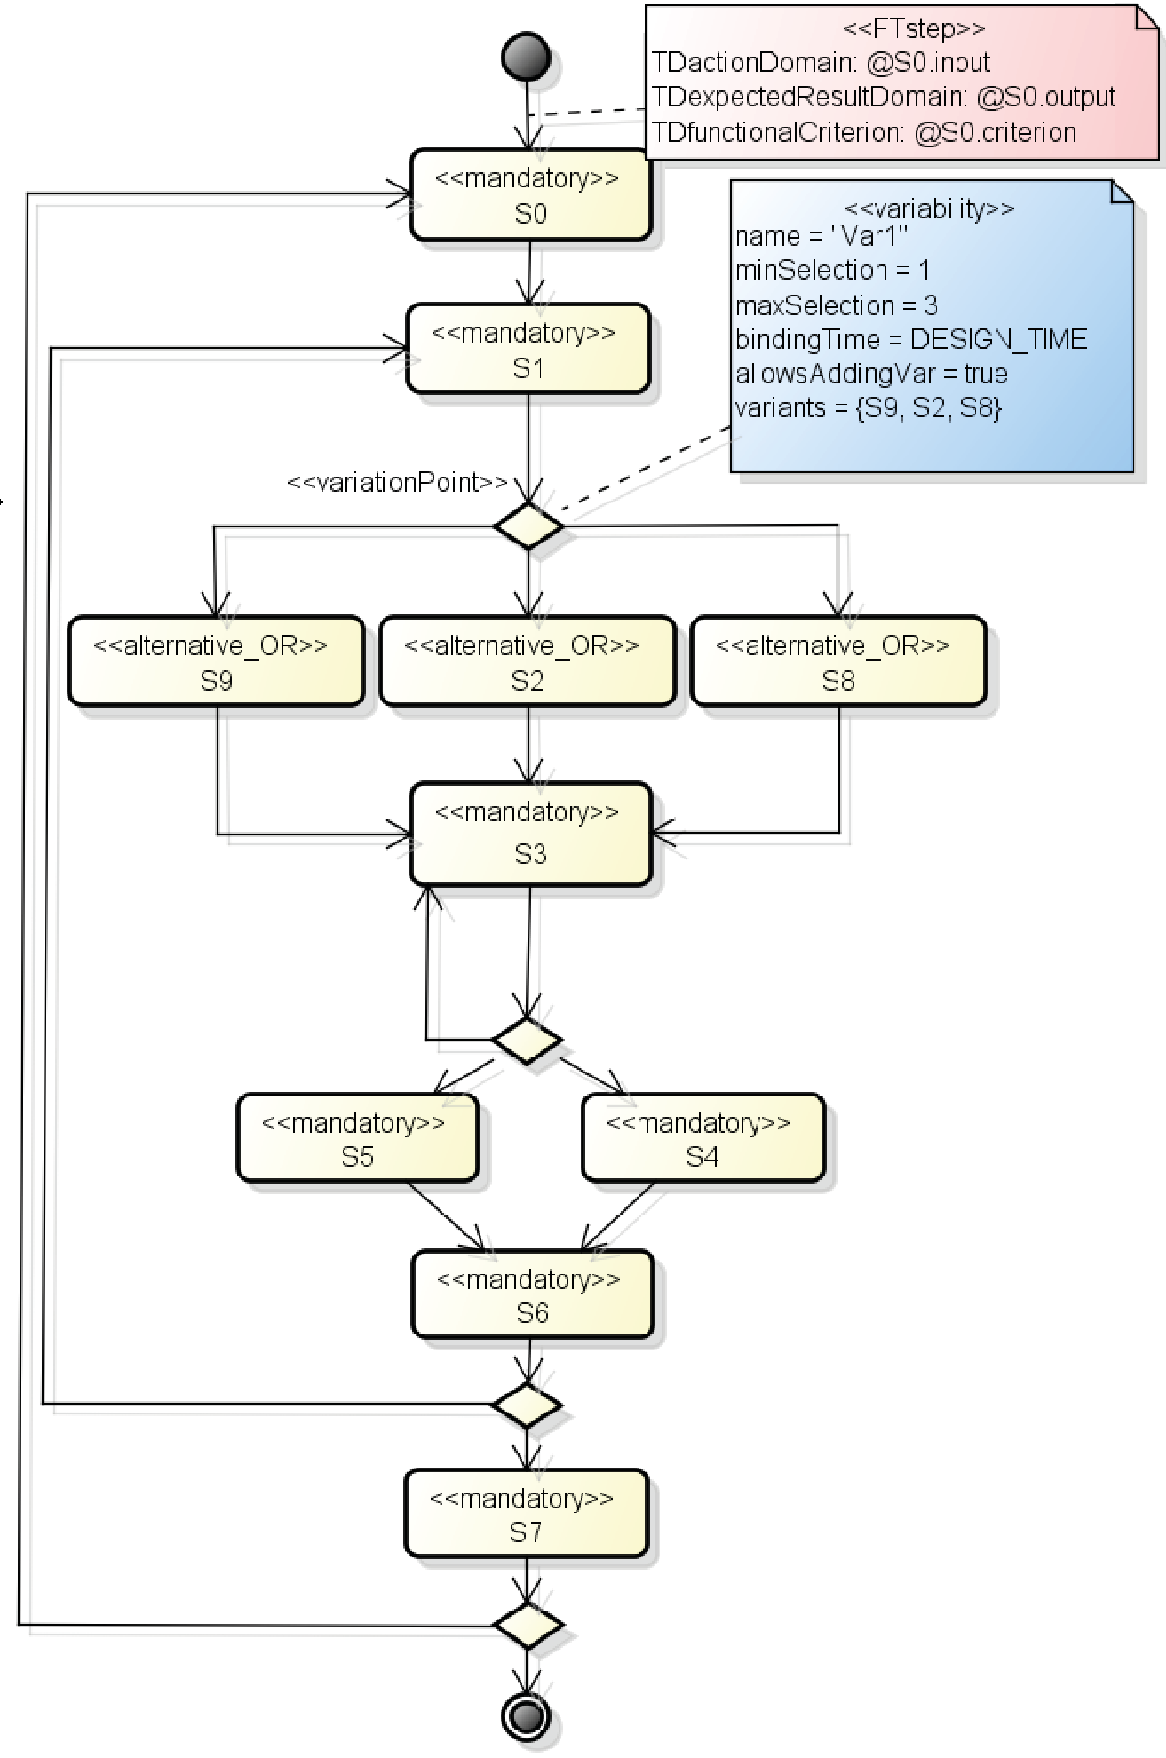
\includegraphics[scale=0.50]{costa1.pdf}
	\caption{Diagrama de atividades \textit{Game Menu} da LPS AGM \cite{costa2016split}}
	\label{fig:costa1}
\end{figure}

Na engenharia de domínio, um DA é convertido em uma MEF que é estendida para lidar com informações sobre variabilidade, exemplificado pela \ref{fig:costa3}. Em seguida, se faz a utilização de um modelo de geração de sequência de teste que foi codificado, denominada \textit{Harmonized State Identifiers} (HSI), a qual realiza a geração das sequências de teste que são armazenadas em um repositório para utilização/reutilização, porém, ainda sem a resolução das variabilidades.

\begin{figure}[h!]
	\centering
	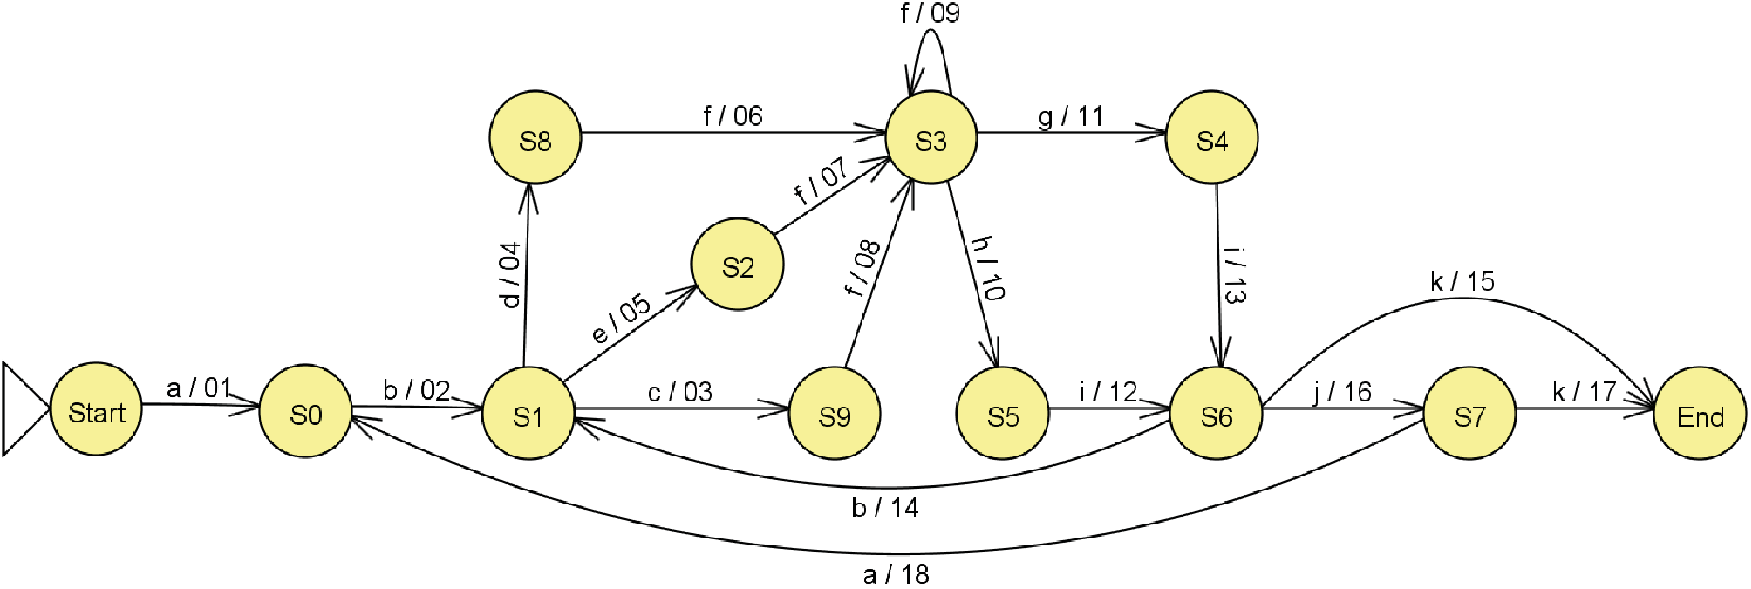
\includegraphics[width=\textwidth]{costa3.pdf}
	\caption{Representação da MEF gerada a partir do DA da \ref{fig:costa1} \cite{costa2016split}}
	\label{fig:costa3}
\end{figure}

\begin{table}[h!]
	\centering
	\caption{Sequência de teste gerada a partir da \ref{fig:costa3}}
	\label{tab:sequencia_teste}
	\begin{tabular}{l|l}
		\hline
		\multicolumn{1}{c}{\textbf{ID}} & \textbf{\begin{tabular}[c]{@{}l@{}}Conjunto de sequência\\ de teste\end{tabular}} \\ \hline
		Sequência1 & ab\{d;e;c\} VP\_or fff, \\ \hline
		Sequência2 & ab\{d;e;c\} VP\_or fgib, \\ \hline
		Sequência3 & ab\{d;e;c\} VP\_or fgik, \\ \hline
		Sequência4 & ab\{d;e;c\} VP\_or fhib, \\ \hline
		Sequência5 & ab\{d;e;c\} VP\_or fhik, \\ \hline
		Sequência6 & ab\{d;e;c\} VP\_or fgijk, \\ \hline
		Sequência7 & ab\{d;e;c\} VP\_or fgijab \\ \hline
	\end{tabular}
\end{table}

\subsection{Métodos de Geração de Casos de Teste}
\label{cap2subsec:metodo_geracao}

Métodos de geração de casos de teste têm por objetivo verificar se uma implementação está correta em relação à especificação, por meio da execução de atividades de teste e validação em sistemas descritos por modelos \cite{fujiwara1991test}, para isso, devem ser geradas sequências de testes.

Apesar dos métodos definirem procedimentos para a geração de testes, a principal diferença que os evidenciam é o custo da geração dessas sequências e a capacidade de detecção de defeitos (efetividade). Dessa  forma,  deve-se  levar  em  conta  a  relação  custo-benefício  de  cada  método \cite{pinheiro2012subsidios}. 

O foco principal consiste em promover a detecção do maior número possível de defeitos existentes em uma implementação, levando em conta o tamanho do conjunto gerado, para que não inviabilize a sua aplicação prática. 

Os métodos de geração são fortemente baseados em sequências básicas, assim, são apresentados de forma simplificada os métodos de geração de sequências de teste mais utilizados na academia:

\begin{itemize}
	\item \textit{State Cover} (Q);
	\item \textit{Transition Cover} (P);
	\item Sequência de Separação (SS);
	\item Sequência de Distinção (DS);
	\item Sequência Única de Entrada e Saída (UIO);
	\item Conjunto de Caracterização (W);
	\item Conjunto de Identificação (Wp); e
	\item Conjunto de Identificadores Harmonizados (Hi).
\end{itemize}

Considerando essas sequências básicas, os métodos de geração utilizam em sua base uma ou várias dessas sequências. A seguir são discutidos, de forma objetiva, os métodos utilizados para a geração dos casos de teste.

\subsubsection{Método TT}

O método  \textit{Transition Tour} (TT), proposto por \citet{naito1981fault}, consiste em construir uma sequência que percorra pelo menos uma vez todas as transições de uma MEF. \citet{sidhu1989formal} definem uma \textit{Transition Tour} como sendo uma sequência de teste que pode ser gerada simplesmente aplicando entradas aleatórias em uma MEF, a partir do estado inicial, até que todas as transições tenham sido cobertas, finalizando no estado inicial. Porém, como a geração é aleatória, muitas sequências redundantes podem ser geradas. Assim, métodos de redução devem ser aplicados para eliminar as redundâncias presentes na sequência final.

\subsubsection{Método W}

Um dos métodos mais difundidos para geração de sequências de testes, o método \textit{Auto-mata Theoretic} ou, como ficou mais conhecido, Método W foi proposto por \citet{chow1978testing}. O nome atribuído ao método originou-se por causa da referência feita por \citet{chow1978testing} ao conjunto de caracterização, utilizado pelo método, como conjunto W. O método W pode ser considerado um método clássico e precursor da área, uma vez que a maioria dos trabalhos seguintes foram baseados no método W. Uma restrição quanto ao método é em relação à sua aplicabilidade, que exige que as MEFs sejam: determinísticas, completas, inicialmente conexas e minimais.


\subsubsection{Método WP}

O método W parcial (Wp), do inglês \textit{partial W}, foi proposto por \citet{fujiwara1991test} como uma melhoria do método W. A partir do conjunto W é criado o conjunto de identificação Wi, que extrai um subconjunto do conjunto W capaz de identificar cada estado da MEF, dependendo do estado final \textit{si} que foi alcançado pela sequência.  

\subsubsection{Método DS}

O método DS é baseado na sequência de distinção DS e foi proposto inicialmente por \citet{hennine1964fault} com a utilização de sequências SS para gerar uma sequência de verificação em conjunto com a DS. \citet{gonenc1970method} apresenta a opção de se utilizar grafos para a geração das sequências.

Os demais trabalhos foram desenvolvidos com o intuito de diminuir o tamanho da sequência de verificação, utilizando a modelagem baseada em grafos proposta por \citet{gonenc1970method}. A aplicabilidade do método é condicionada a existência da sequência DS, uma vez que nem todas as MEFs a possuem. Além disso, o método DS só é aplicável em MEFs: determinísticas, completas, fortemente conexas e minimais.

\subsubsection{Método UIO}

O método UIO foi originalmente proposto por \citet{sabnani1988protocol} como um método completo. Porém, \citet{vuong1989uiov} apresentou um contra-exemplo que demostrou que o método UIO não garante a cobertura completa de defeitos para todas as MEFs. O método é baseado em sequências UIO e é realizado em apenas uma fase, correspondente à fase dois do método W. Da mesma forma que o método W, a aplicabilidade do método UIO está restrita à existência das sequências UIO e à MEFs que sejam: determinísticas, inicialmente conexas, completas e minimais.  

\subsubsection{Método UIOv}

Como uma variação do método UIO, o método UIOv (\textit{UIO variation}) foi proposto por \citet{vuong1989uiov}. A solução apresentada inclui uma fase a mais no processo de geração de testes, em que seriam aplicadas todas as sequências UIO a todos os estados pelo menos uma vez, ou seja, a sequência UIOi  seria aplicada em cada estado \textit{sj}  atingido a partir do conjunto \textit{Q}, tal que \textit{i={0..n}} e \textit{j={0..n}}.

\subsubsection{Método HSI}
\label{cap2subsubsec:hsi}

O método HSI \cite{petrenko1994nondeterministic}, assim como a maioria dos métodos propostos, foi proposto como uma melhoria para o método \textit{W}. Além de gerar conjuntos de testes completos, o método apresenta um grau de aplicabilidade maior que o das demais métodos, pois pode ser aplicado em MEFs completas e em MEFs parciais. Dessa forma, o método consegue cobrir um número maior de especificações¸ comparado com o método \textit{W}.

Fazendo um paralelo entre os métodos \textit{Wp} e HSI, ambos têm sequências de separação por estado que possuem o objetivo de distinguir o estado \textit{si} dos demais. Dessa forma, a diferença entre os conjuntos \textit{Wi} e \textit{Hi} está na maneira como são construídos. Enquanto \textit{Wi} é obtido a partir do conjunto  \textit{W}, o \textit{Hi} é construído a partir de sequências de separação que distinguem cada par de estados da  MEF.  

Durante a pesquisa sobre as ferramentas de geração de casos de teste mencionadas na Seção \ref{cap3subsec:definicaoabordagem} foram encontrados dois trabalhos que possuíam características compatíveis com os requisitos necessários para a utilização na abordagem proposta nesta dissertação, a ferramenta JPlavisFSM \cite{pinheiro2012jplavisfsm} e a SPLiT-MBt \cite{costa2016split}, ambas realizam o processo de geração de casos de teste considerando MEF. A partir desse cenário, procurou-se avaliar tais ferramentas para verificar a viabilidade de utilização.


\subsection{Ferramenta de Geração de Sequências de Teste JPlavisFSM}
\label{cap2subsec:plavis}

A ferramenta JPlavisFSM \cite{pinheiro2012jplavisfsm} é uma versão atualizada da antiga plataforma PLAVIS, resultado do projeto ``PLAVIS - Plataforma para Validação e Integração de Software em Sistemas Espaciais" \cite{da2008plavis}, financiado pelo Conselho Nacional de Pesquisa (CNPq) e desenvolvido entre os anos de 2002 e 2004. A primeira versão da plataforma integrava outras ferramentas de geração e uma implementação do algoritmo UIO, responsáveis pela geração de casos de teste a partir de MFEs. A referida ferramenta foi integrada a ferramenta ProteumFSM que possuía a capacidade de criar mutantes de especificação em MEFs. A JPlavisFSM faz algo similar que a SPLiT-MBt, porém conforme será apresentado, não atende a todos os requisitos essenciais da abordagem \textit{SMartyTesting}.

A ferramenta permite a criação de grafos que representam MEFs (\ref{fig:plavis}), que posteriormente possam ser utilizados para a criação de sessões de teste. Na geração de sessão de teste a ferramenta dispõe de alguns métodos de geração de sequência (\ref{fig:plavis2}) o que a torna uma ferramenta com grande potencial de recursos.

\begin{figure}[h!]
	\centering
	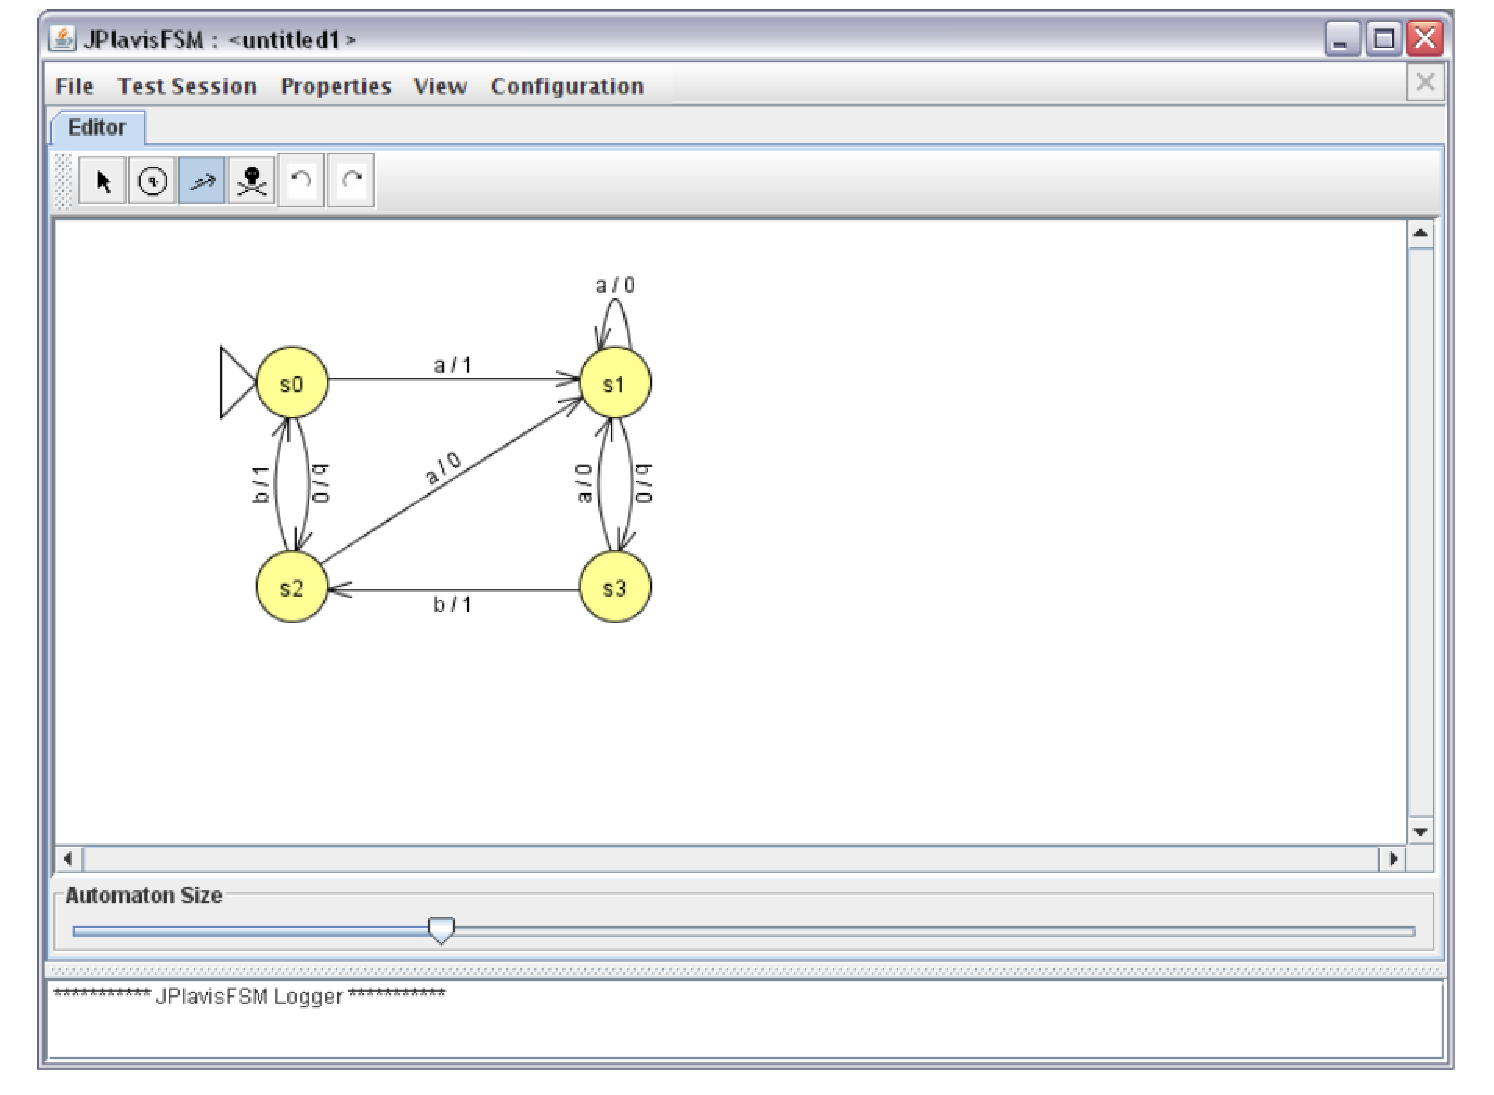
\includegraphics[scale=0.55]{plavis.pdf}
	\caption{representação de uma MEF utilizando a ferramenta JPlavisFSM \cite{pinheiro2012jplavisfsm}}
	\label{fig:plavis}
\end{figure}

\begin{figure}[h!]
	\centering
	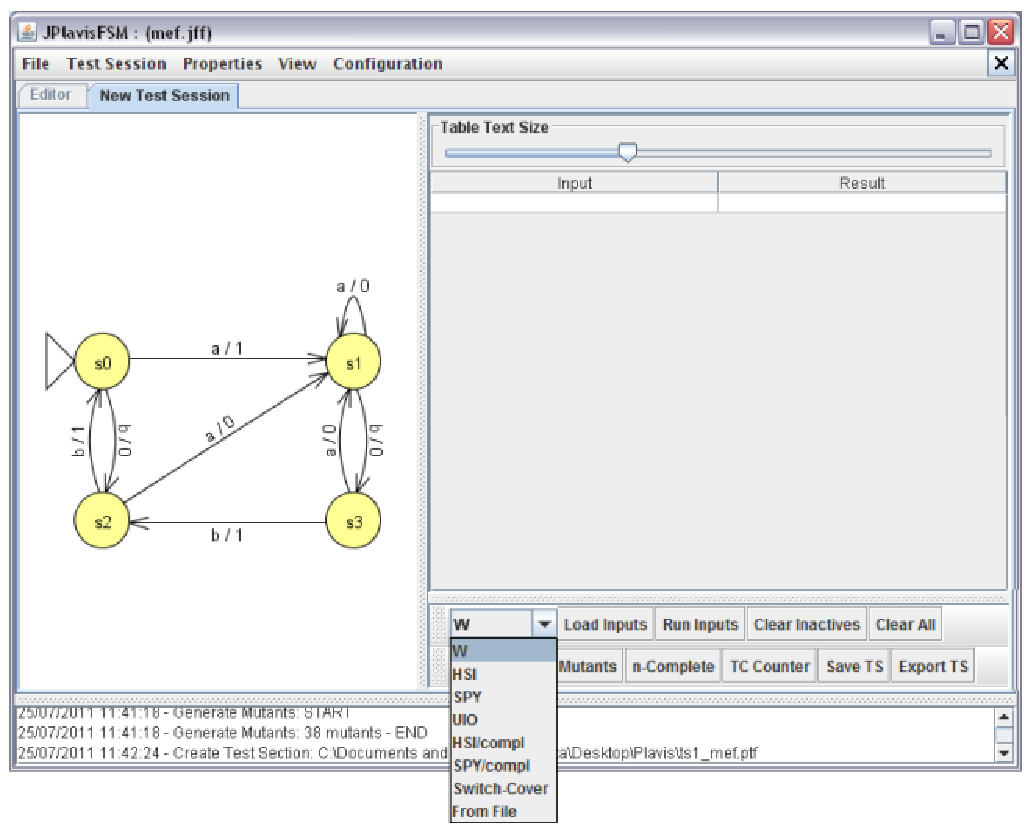
\includegraphics[scale=0.80]{plavis2.pdf}
	\caption{Geração de sequências de teste pela ferramenta JPlavisFSM \cite{pinheiro2012jplavisfsm}}
	\label{fig:plavis2}
\end{figure}

Após comparações entre as duas ferramentas (\ref{tab:splitxplavis}) optou-se por utilizar a SPLiT-MBt como ferramenta de apoio na segunda etapa da abordagem \textit{SMartyTesting}, para apoiar a geração de casos de teste com base nos artefatos de entrada provenientes da primeira etapa. 

\begin{table}[h!]
	\centering
	\caption{Comparação de requisitos SPLiT-MBt e JPlavisFSM}
	\label{tab:splitxplavis}
	\begin{tabular}{l|c|c}
		\hline
		\multicolumn{1}{c}{Requisito} & SPLiT-MBt & JPlavisFSM \\ \hline
		Suporte à variabilidade & Sim & Não \\ \hline
		Compatível com LPS & Sim & Sim \\ \hline
		\begin{tabular}[c]{@{}l@{}}Formato de artefato\\ de  entrada\\ compatível com o requisito\end{tabular} & Sim & Não \\ \hline
		\begin{tabular}[c]{@{}l@{}}Suporte a método\\ de geração  de sequência \\de teste\end{tabular} & Sim & Sim \\ \hline
		Compatível com SMarty & Sim & Não \\ \hline
	\end{tabular}
\end{table}

\section{Diagramas de Sequência e de Atividades}
\label{cap2sec:sequenciaatividade}

A UML (\textit{Unified Modeling Language}) é uma linguagem-padrão para a elaboração da estrutura de projetos de software. Pode ser empregada para a visualização, a especificação, a construção e a documentação de artefatos que façam uso de sistemas complexos de software \cite{booch2006uml}.

Na linguagem UML faz-se uso de diagramas para a modelagem de sistemas, onde, para cada nível de interpretação e criação dispõe um diagrama com finalidade diferente. Quando se fala em modelagem de aspectos dinâmicos de sistemas, é possível mencionar os diagramas de atividades e sequência, onde a atividade mostrando o fluxo de controle de uma atividade para outra, apresentando a concorrência bem como, as ramificações de controle, \ref{fig:DA}.

\begin{figure}[h!]
	\centering
	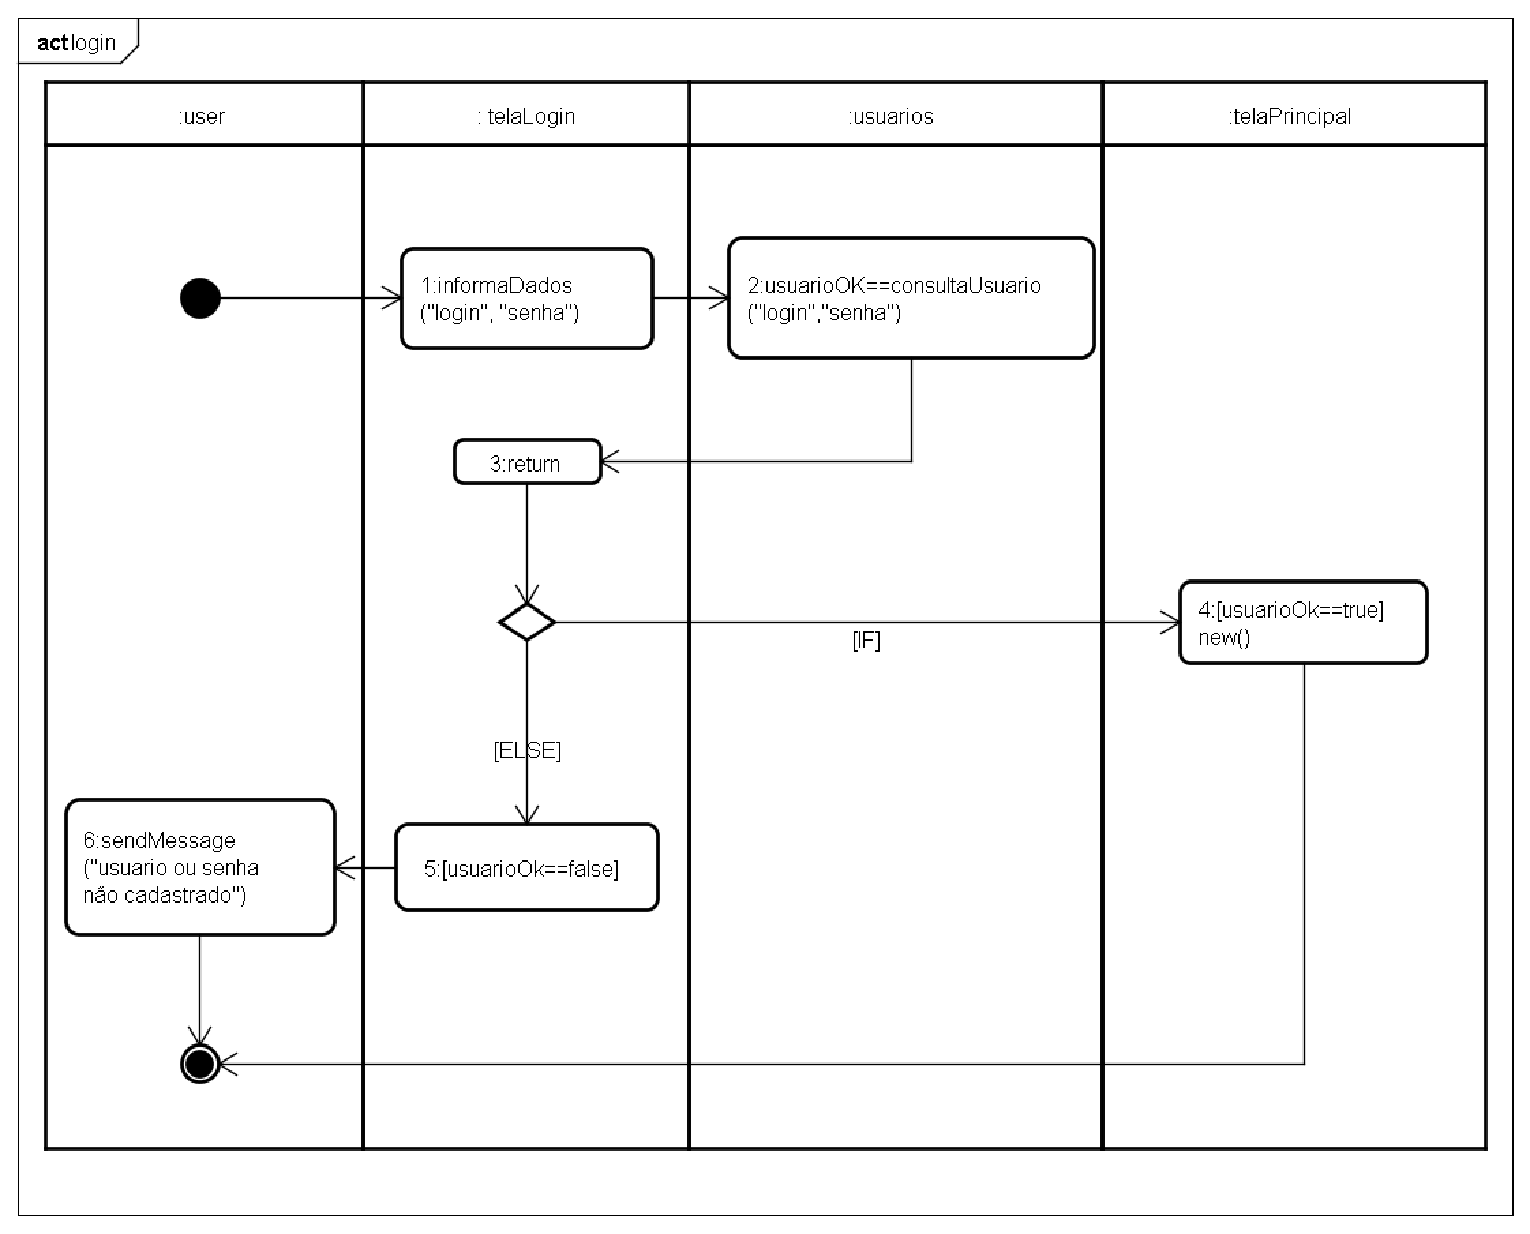
\includegraphics[scale=0.60]{login_exemple_da.pdf}
	\caption{Exemplo de um diagrama de atividades}
	\label{fig:DA}
\end{figure}


O diagrama de sequências é um diagrama de interação, formado por um conjunto de objetos e seus relacionamentos, incluindo mensagens que poderão ser enviadas entre eles. O DS dá ênfase à ordenação temporal das mensagens e a estrutura dos objetos. (\ref{fig:DS})

\begin{figure}[h!]
	\centering
	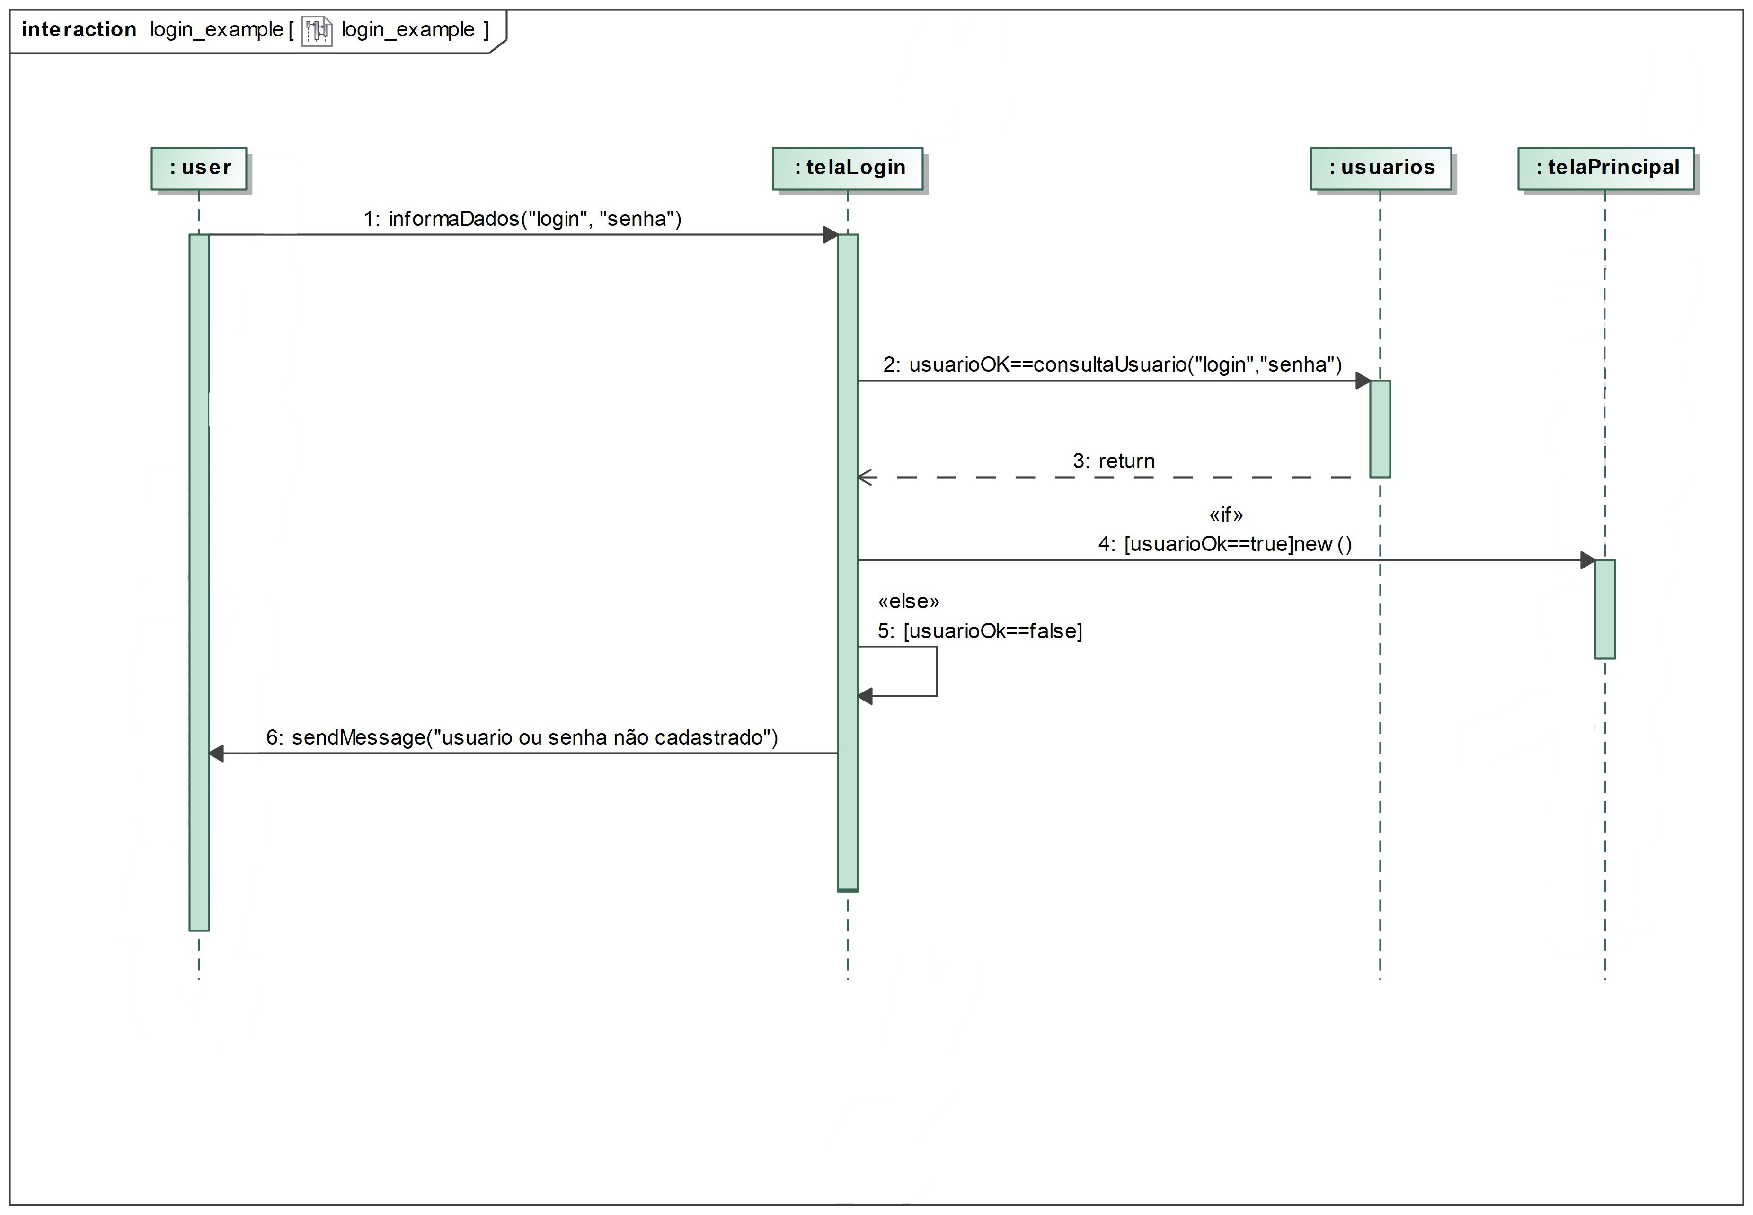
\includegraphics[scale=0.50]{login_example_ds.pdf}
	\caption{Exemplo de um diagrama de sequência}
	\label{fig:DS}
\end{figure}


Por isso, pode se concluir que diagramas de atividades possuem um nível maior de abstração se comparados ao diagrama de sequência, que fica mais próximo à classe do sistema, demonstrando comportamentos de objetos, enquanto que o de atividades, demonstra os fluxos e direções que cada atividade do sistema seguirá.

Essa seção apresenta a aplicação para cada diagrama aqui mencionado, dado que ambos fazem parte deste trabalho de dissertação, \textit{SMartyTesting} fazendo uso de diagramas de sequência em comparação à SPLiT-MBt, que faz uso de diagramas de atividades.

\section{Considerações Finais}
Neste tópico foram apresentados todos os elementos que são considerados importantes para fundamentar esta dissertação, como os conceitos de LPS e a abordagem \textit{SMarty}, assim como, os conceitos e aplicação de TBM para LPS e, por último, a abordagem SPLiT-MBt.
